\documentclass[11pt,letterpaper]{article}
\usepackage{libertinus-otf}
\usepackage{amsmath,amsthm}
\usepackage[margin=1in,headheight=15pt]{geometry}
\usepackage{graphicx,booktabs,array,longtable,tabularx}
\usepackage{microtype,enumitem,xcolor,fancyhdr}
\usepackage{titlesec}
\usepackage[numbers,sort&compress]{natbib}
\usepackage[unicode,colorlinks=true,linkcolor=ink,citecolor=ink,urlcolor=ink]{hyperref}
\definecolor{ink}{HTML}{243E52}
\definecolor{muted}{HTML}{59656E}
\definecolor{accent}{HTML}{A45C36}
\hypersetup{pdftitle={Asset Price Bubbles: Theory, Signals, and Traded Contracts},pdfauthor={Research manuscript},pdfsubject={Rebalancing, identification, daily and intraday monitoring, options and baskets}}
\urlstyle{same}
\linespread{1.035}
\setlength{\parskip}{0.3em}
\setlength{\parindent}{1.1em}
\setlength{\emergencystretch}{2em}
\setlength{\tabcolsep}{5pt}
\renewcommand{\arraystretch}{1.17}
\setlist{nosep,leftmargin=*,topsep=0.4em}
\clubpenalty=10000 \widowpenalty=10000
\allowdisplaybreaks
\newcolumntype{L}[1]{>{\raggedright\arraybackslash}p{#1}}
\newcolumntype{Y}{>{\raggedright\arraybackslash}X}
\titleformat{\part}[display]{\color{ink}\centering\Huge\bfseries}{\Large Part \Roman{part}}{0.5em}{}
\titleformat{\section}{\color{ink}\Large\bfseries}{\thesection}{0.6em}{}
\titleformat{\subsection}{\large\bfseries}{\thesubsection}{0.6em}{}
\titlespacing*{\section}{0pt}{2.3ex plus 1ex}{1ex}
\titlespacing*{\subsection}{0pt}{1.8ex plus 1ex}{0.7ex}
\pagestyle{fancy}
\fancyhf{}
\fancyhead[L]{\small\color{muted}Asset Price Bubbles}
\fancyhead[R]{\small\color{muted}\nouppercase{\leftmark}}
\fancyfoot[C]{\thepage}
\renewcommand{\headrulewidth}{0.25pt}
\renewcommand{\sectionmark}[1]{\markboth{\thesection\quad #1}{}}
\newtheorem{theorem}{Theorem}
\newtheorem{proposition}[theorem]{Proposition}
\newtheorem{corollary}[theorem]{Corollary}
\theoremstyle{definition}
\newtheorem{example}[theorem]{Example}
\newcommand{\E}{\mathbb{E}}
\newcommand{\Prob}{\mathbb{P}}
\newcommand{\R}{\mathbb{R}}
\newcommand{\ind}{\mathbf{1}}
\newcommand{\dd}{\,\mathrm{d}}
\newcommand{\scope}[1]{\par\smallskip\noindent\textit{Scope.} #1\par}
\newcommand{\source}[1]{\par\smallskip{\footnotesize\noindent\textit{Research record:} #1.\par}}
\newcommand{\tablerows}[1]{\csname @@input\endcsname #1 }
\newcommand{\partopening}[3]{\clearpage\part{#1}\label{#2}\noindent\textit{#3}\par\medskip}
\begin{document}
\begin{titlepage}
\thispagestyle{empty}
\vspace*{1.0in}
{\color{accent}\large RESEARCH MANUSCRIPT\par}
\vspace{0.4in}
{\color{ink}\fontsize{34}{39}\selectfont\bfseries Asset Price Bubbles\par}
\vspace{0.22in}
{\color{ink}\LARGE Theory, Signals, and Traded Contracts\par}
\vspace{0.5in}
{\large Rebalancing and identification\par
Daily and intraday monitoring\par
Leveraged funds, options, and constituents\par}
\vfill
\noindent A unified account of the research, with economic explanations,
principal mathematical results, and evidence from simulations and market data.
\par\bigskip
\noindent Draft prepared 9 October 2026\par
\noindent Evidence through the research snapshot documented in Appendix~\ref{app:record}.
\end{titlepage}
\pagenumbering{roman}
\markboth{Overview}{}
\section*{Abstract}
\phantomsection
\addcontentsline{toc}{section}{Abstract}
In the strict-local-martingale theory of asset prices, a bubble is a
shortfall of expected future value under a pricing measure relative to the
current price. This manuscript studies how that valuation concept relates
to patterns in observed prices and to the wealth produced by trading
strategies. We classify constant-proportion wealth by exposure and the
asset's behavior near zero and at very high prices. Continuous rebalancing
can create a strict local martingale from a true-martingale asset, and the
classification can reverse when rebalancing occurs on a finite grid. We
also establish limits on identification from price paths and examine what
liquidation rules, option contracts, and constituent information add to
the valuation problem.

The empirical work develops daily and intraday signals of return variance
rising with the price level. This pattern has a connection to bubble
mechanisms in both local-volatility and stochastic-volatility models.
The measurement problem is to distinguish it from changes in background
volatility. The daily method uses a predictable market volatility scale;
the intraday method compares price movements within each session while
updating its background state between sessions. We evaluate the methods
in simulations and historical records, with particular attention to how
calibration changes their alarm patterns.

The results show substantial sensitivity in the intended simulation
families and distinct behavior on market data. In shared-market-scale
and constant-elasticity simulations, the daily statistic detects 39--72\%
of the specified alternatives, compared with 7--14\% for a calibrated
explosive-price benchmark. It remains relatively quiet in crisis cohorts
and flags all four studied homebuilders about 400 trading sessions before
their 2005 peaks, versus one for the benchmark. The intraday score adds
out-of-sample drawdown information to that benchmark. These findings
support the signals as measurements of price--variance behavior, with
the theory specifying the additional assumptions needed to interpret
such behavior as a pricing bubble.

\section*{How to read the manuscript}
\phantomsection
\addcontentsline{toc}{section}{How to read the manuscript}
The four parts answer different questions within one framework.
Part~\ref{part:theory} defines the economic object and establishes what
rebalancing and observation can change. Part~\ref{part:signals} introduces the
proposed signals, their calibration, and their daily and intraday evidence.
Part~\ref{part:funds} follows the theory into finite trading and liquidation.
Part~\ref{part:options} asks what options and index constituents add to prices
alone. A reader interested primarily in monitoring can begin with
Section~\ref{sec:targets}, then read Part~\ref{part:signals}; the preceding
theory explains the limits on interpretation.

Section~\ref{sec:literature} introduces the relevant literature and explains
how the contributions build on it. The main text includes the short arguments that explain the results. Longer
derivations, implementation specifications, and the research-to-manuscript map
are in the appendices. Experiment numbers identify reproducible research
records, not a sequence the reader must follow. No new empirical experiment is
introduced in this manuscript: the tables and figures reorganize existing
results. The selected generated tables are read directly from the stored
experiment summaries at build time.

\clearpage
\tableofcontents
\clearpage
\pagenumbering{arabic}
\section{The questions and the contributions}\label{sec:targets}
An investor confronted with a rapidly appreciating stock might ask whether
the price is detached from fundamental value, whether volatility rises as
the price rises, whether a crash is becoming more likely, and whether a
leveraged position changes those risks. These questions concern different
aspects of the same episode. Understanding their connections helps determine
what to measure and how to interpret the result.

We focus on a particular pattern: return variance increasing with the price
level. It appears in models where the price is a strict local martingale,
and it offers something concrete to look for in market data. Measuring it
requires separating movements associated with the stock's price from changes
in market conditions and background volatility. The daily and intraday
signals developed here make that separation in different ways. Alongside
them, the theoretical analysis explains how the bubble concept changes
when we move from an asset to a rebalanced portfolio or an option contract.

Our starting point is the strict-local-martingale definition of a bubble
\cite{jarrow2007complete}. In discounted units, under a specified pricing
measure $Q$, a nonnegative local martingale $S$ is a supermartingale. Its
finite-horizon defect is
\begin{equation}\label{eq:defect}
 b_S(T)=S_0-\E_Q[S_T]\geq0.
\end{equation}
A positive defect means that $S$ fails to be a true martingale on that horizon.
The physical measure $P$ describes the distribution from which historical
observations are drawn. An expectation under $Q$ is a valuation object, not an
estimate of the investor's average realized return under $P$.

A widely used approach to monitoring bubbles looks for explosive price
growth: intervals on which prices behave like an autoregression with a
root greater than one. The generalized supremum augmented Dickey--Fuller
test (GSADF) is a prominent example \cite{phillips2012multiple}. We use an
empirically calibrated version as a benchmark. Its focus on price dynamics
provides a useful comparison with our focus on the relationship between
price and return variance. A third question, whether a signal predicts a future drawdown,
concerns outcomes under $P$. The literature already documents that large
run-ups and their characteristics can carry crash information without run-ups
necessarily predicting low average returns \cite{greenwood2017bubbles}.
Forecasting is therefore one way to examine usefulness, not the definition of
the object studied here.

\begin{table}[htbp]
\centering\small
\begin{tabularx}{\linewidth}{@{}L{0.22\linewidth}YY@{}}
\toprule
Object & Evidence it requires & What a positive finding means \\
\midrule
Pricing defect & A pricing law and a valuation convention & A shortfall of
terminal expectation relative to current value \\
Explosive behavior & A specified time-series null and calibration & Departure
toward explosive price dynamics in that testing framework \\
Price-level variance dependence & A variance model, nuisance treatment, and
calibration & An observed pattern better fitted by positive level dependence \\
Future loss risk & A forecast design and genuinely later outcomes & An
association with losses over a specified horizon \\
\bottomrule
\end{tabularx}
\caption{Four questions often grouped under the word ``bubble.'' A result in
one row does not automatically establish a result in another.}
\label{tab:objects}
\end{table}

\subsection{What this research adds}
The theoretical centerpiece is a classification of constant-proportion
wealth. An investor who continually restores a fixed fraction of wealth
to an asset can inherit its strictness or acquire strictness through a
different mechanism: rebalancing into an asset that can reach zero.
The result depends on exposure and on the asset's behavior at both ends
of its price range. Finite rebalancing and liquidation change the answer,
which gives the classification a direct interpretation for traded funds.
The result applies established martingale criteria; its prior-art comparison
is incomplete, and we make no separate novelty claim for the finite-trading
results.

The identification results explain what observed prices can contribute to
that theory. A finite record reveals behavior within a visited range, while
the martingale classification can depend on an unvisited tail. Stochastic
volatility adds another connection and another distinction. In Sin's model,
positive alignment of price and volatility shocks is central to strictness,
but different pricing measures can give the same observed law different
valuation implications. These results motivate measuring price--variance
association while keeping its statistical and valuation interpretations
explicit.

The methodological contribution is a pair of daily and intraday signals
built around that association. Both compare positive and nonpositive level
dependence using the same background-variance specification. The daily
method adjusts for recent market volatility, leaving the stock's own level
available to explain additional variation. The intraday method anchors
prices within each session and updates its background state between
sessions. Their construction addresses a recurring measurement problem:
a sufficiently flexible volatility adjustment can absorb the pattern we
want to detect.

The empirical contribution is an evaluation of those choices, including
simulation sensitivity, calibration, historical alarms, and a supplementary
forecasting comparison. In the shared-market-scale simulations and a
constant-elasticity diffusion family, the daily statistic detects roughly
39--72\% of the specified alternatives, against 7--14\% for calibrated
GSADF. In historical data, its sparse crisis-cohort alarms coexist with a
coherent early signal across D.R. Horton, Lennar, Pulte, and Toll Brothers,
all around 400 sessions before their 2005 peaks. The intraday score adds
modest out-of-sample drawdown information to GSADF. Part~\ref{part:signals}
presents these findings alongside the settings where each method is weaker.
Calibration is part of the result: the reference distribution determines
what counts as unusual and can materially change the resulting alarms.

\subsection{How to assess the evidence}
The principal distinction is between a pricing defect under $Q$ and a
measured pattern under $P$. Simulation detection rates have known generating
models; historical episode and calm-control labels are comparison groups.
Reported calibration and forecast results describe the evaluated procedures
and populations. Across those comparisons, GSADF remains the stronger general
run-up benchmark, the intraday score contributes incremental drawdown
information, and the daily statistic's contribution is its sensitivity and
selective historical alarm pattern rather than a demonstrated forecasting
gain.

The research used retrospective episodes and current-constituent universes,
with overlapping windows and repeated method development. Chronological
out-of-sample fits therefore test temporal transfer within this research
record, rather than an untouched research holdout. These shared qualifications
apply throughout the empirical part. More specific limitations are stated
where they change the interpretation of a result.

\section{Background and relation to existing work}\label{sec:literature}
The literature approaches bubbles through several different observable
features: prices relative to cash flows, explosive growth, volatility that
increases with the price level, and run-ups followed by crashes. Each approach
starts from an economic mechanism and then asks which implications can be
measured. The present research connects the strict-local-martingale approach
to practical monitoring and to traded contracts. Its closest predecessors
therefore include both mathematical valuation papers and empirical detection
methods.

\subsection{From fundamental value to a pricing defect}
In the classical present-value formulation, an asset's fundamental value is
the discounted value of its future cash flows. A bubble is an additional
price component consistent with the pricing equation but not explained by
those cash flows. Empirical tests must consequently specify the cash-flow
process and the way investors discount it. G\"urkaynak's survey explains why
this creates an identification problem: evidence attributed to a bubble can
also be explained by changes in fundamentals or discounting
\cite{gurkaynak2005econometric}. A striking price path alone does not resolve
that comparison.

The strict-local-martingale literature provides a precise continuous-time
valuation framework. Cox and Hobson study prices that are local martingales
under a pricing measure but lose expectation, including local-volatility
and feedback models \cite{cox2005local}. Jarrow, Protter, and Shimbo place
such behavior in a theory of asset-price bubbles and market completeness
\cite{jarrow2007complete}. In the finite-horizon, discounted setting used
here, the object is the defect in \eqref{eq:defect}. This makes the
mathematical question explicit: under which models and trading rules does
current value exceed expected terminal value under the specified pricing law?

The specification of that law matters in an incomplete market. Herdegen
and Schweizer define fundamental value through superreplication and develop
a symmetric treatment of assets and numeraires. Their strong-bubble concept
differs from a bubble defined under one chosen equivalent local martingale
measure; their Example~5.5 explicitly exhibits different martingale behavior
under two such measures \cite{herdegen2016strong}. Our results concern the
fixed-measure defect. The contribution of the identification analysis is to
make the implications for observation precise: tail completions and changes
of pricing measure can preserve the available price information while
changing that defect.

\subsection{What volatility can reveal about a bubble}
Jarrow, Kchia, and Protter offer the closest methodological starting point
for the signals in this manuscript \cite{jarrow2011detect}. For a suitable
driftless diffusion $\dd S_t=\sigma(S_t)\dd W_t$, strictness is governed by
the upper-tail integral
\[
 \int_c^\infty \frac{x}{\sigma^2(x)}\dd x.
\]
The economic idea is that sufficiently rapid growth of volatility at high
prices can generate a pricing defect. Their detection procedure estimates
the diffusion coefficient from observed prices and then assesses its tail
behavior. They explicitly identify the extrapolation problem and propose
parametric and reproducing-kernel methods for extending the estimate beyond
the observed range.

Nonparametric diffusion estimation supplies the local measurement tools.
Florens-Zmirou studies estimation from discretely observed paths;
Bandi and Phillips develop nonparametric methods using occupation-time
information \cite{florenszmirou1993estimating,bandi2003fully}. Repeated visits
to a price region provide information about volatility there. More frequent
observations improve that local information, but need not reveal how the
coefficient behaves at prices never reached. Obayashi, Protter, and Yang
extend the detection approach toward dating bubble episodes: they construct
daily signals from intraday observations and smooth the noisy classifications
with a hidden Markov model \cite{obayashi2015lifetime}. Thus both
volatility-based detection and the use of intraday data to produce a daily
monitor have clear precedents.

Our theory specifies exactly what remains undetermined when the coefficient
is known only on a visited interval, including the lower endpoint that
matters for rebalanced wealth. The testing results then turn this observation
into a statistical statement: within the stated model classes, a
true-martingale completion can approximate the observed law of a strict
local martingale arbitrarily well. These are precise formulations of an
existing identification concern, with consequences for what assumptions a
useful test must impose.

The empirical methods take a more local target. They measure whether
\emph{return variance} rises with the price level after accounting for a
declared background scale. For intuition, if $\sigma(x)=a x^p$, then return
variance is $a^2x^{2(p-1)}$. The positive exponent estimated by a signal is
therefore connected to the classical tail mechanism, while remaining an
observable feature of the fitted window. Our methodological contribution is
the construction of that measurement under changing market volatility,
together with its calibration and comparative evidence. It is a different
use of the volatility insight from extrapolating a fitted coefficient to
infinity.

\subsection{Explosive prices, episode dating, and crash risk}
Another influential approach asks whether prices exhibit temporarily
explosive autoregressive dynamics. In a simple representation, the question
is whether the coefficient in $y_t=\rho y_{t-1}+u_t$ exceeds one over some
interval. The generalized supremum augmented Dickey--Fuller test scans
windows with varying starting and ending dates. This flexibility lets it
detect multiple episodes that a test tied to one starting date may miss;
the associated backward-window statistics support episode dating
\cite{phillips2012multiple,phillips2013realtime}. Panel methods can gain
information by grouping series with similar explosive behavior
\cite{liu2022panel}.

These tests give a natural practitioner benchmark because they formalize
the familiar pattern of accelerating prices. Their statistical target is
different from the tail condition above: explosive conditional-mean
dynamics and price-dependent conditional variance can appear separately.
This distinction makes the comparison informative. It lets us ask whether
the proposed variance signals detect patterns that an explosive-price
statistic tends to miss, and whether those patterns occur in different
historical episodes.

Volatility adjustment is already an important part of the explosive-testing
literature. Kurozumi, Skrobotov, and Tsarev construct a time transformation
to handle nonstationary volatility and recover a pivotal limiting null
distribution \cite{kurozumi2021time}. Our findings about the calibration
of GSADF belong in that context. The empirical comparisons here evaluate
the specified GSADF implementation and its calibrated thresholds; they
are not comparisons against every volatility-robust extension. The
distinctive evidence is the side-by-side behavior of a variance signal
and an explosive-price benchmark under common simulation and historical
designs.

A further strand studies what happens after observed run-ups. Greenwood,
Shleifer, and You find that sharp increases do not generally imply low
subsequent average returns, but do imply higher crash probabilities;
characteristics such as volatility, turnover, and issuance help distinguish
the outcomes \cite{greenwood2017bubbles}. This is the relevant precedent
for our supplementary drawdown comparison. The intraday result adds
information beyond the GSADF score in the reported forecasting design.
Its contribution is that particular incremental comparison, rather than
the general proposition that volatility or run-up characteristics can
predict crashes.

\subsection{Separating price dependence from background volatility}
Financial volatility changes over time and responds asymmetrically to
returns. Glosten, Jagannathan, and Runkle provide an influential model of
that asymmetry \cite{glosten1993relation}. Such dynamics matter here
because an observed price--variance association can arise through the
joint evolution of prices and a separate volatility state. A useful
measurement procedure must specify which variation its background model
explains and which variation remains available to the price-level term.

The connection to stochastic-volatility bubble theory is also substantive.
In Sin's model, positive alignment of price and volatility shocks can
produce strict-local-martingale behavior; the same model also illustrates
the role of the pricing measure \cite{sin1995complications}. Price--volatility
association is consequently of interest beyond one-dimensional local
volatility. The simulations in this research examine how the signals respond
to both structural level dependence and correlated volatility shocks.
That response helps explain what the statistic measures across model
families.

The daily construction uses a predictable market volatility scale and
compares positive and nonpositive price-level dependence with the same
nuisance specification. The intraday construction anchors the price
within each session and updates the background state between sessions.
These choices preserve a distinction between movements inside the
measurement window and changes in the background scale. Their value is
assessed through simulation, historical alarm patterns, and calibration
transfer. This is the central methodological addition to the earlier
volatility-estimation approach.

The statistical tools used to assess evidence also have established
antecedents. Split-likelihood universal inference supplies a way to
construct finite-sample evidence by estimating an alternative on separate
data and bounding the null likelihood \cite{wasserman2019universal}.
The e-BH procedure controls false discovery rate from valid e-values
under arbitrary dependence \cite{wang2020false}. Rank calibration uses
exchangeability to compare a new score with reference scores
\cite{tibshirani2019conformal}. We apply these ideas to specified
observation models and distinguish their guarantees from the empirical
reference calibration used by the practical scores. The findings about
how calibration changes sensitivity and historical alarms are part of
the contribution, alongside the score designs themselves.

\subsection{Investment, rebalancing, and leveraged funds}
A bubble in an asset raises a separate question about the wealth generated
by trading it. Herdegen and Herrmann connect strict local martingales with
a generalized Johansen--Ledoit--Sornette crash model and solve a power-utility
investment problem. Under their assumptions, investors with relative risk
aversion above one continue to hold the bubble when instantaneous expected
returns are positive \cite{herdegen2013strict}. This gives a useful
investment perspective: the existence of a bubble does not by itself
determine an optimal position. Their crash model also connects the
strict-local-martingale literature to the separate tradition of modeling
log-periodic behavior before crashes.

Our investment question concerns a prescribed rule: keep a constant fraction
of wealth in the asset. The tools are established martingale and diffusion
criteria. Mijatovi\'c and Urusov give the stochastic-exponential criterion
we apply, while Karatzas and Ruf analyze the auxiliary drift family that
arises in the calculation \cite{mijatovic2010martingale,karatzas2015distribution}.
The result developed here classifies the exposure rule across both price
endpoints. In particular, continuous buying into an asset approaching zero
can create strictness in wealth even when the asset is a true martingale.
The comparison with finite trading makes the economic importance of that
boundary mechanism concrete.

For leveraged exchange-traded funds, Avellaneda and Zhang establish the
path dependence of multi-period returns and their relationship to realized
variance, financing, and expenses \cite{avellaneda2009path}. That work
explains why a fund's cumulative return differs from a fixed multiple of
the underlying's cumulative return. Part~\ref{part:funds} addresses a
complementary issue: how finite rebalancing, nonnegativity, and liquidation
affect the martingale classification. The empirical tracking-cost evidence
then places those idealized wealth processes beside observed funds. The
established variance-drag explanation and the endpoint classification
answer different questions about the same trading rule.

\subsection{What options and constituents add}
The option-pricing consequences of strict local martingales are already
central to Cox and Hobson: familiar put--call parity and European--American
relations can change, and admissible trading strategies affect valuation
\cite{cox2005local}. Carr, Fisher, and Ruf develop a joint-superreplication
framework that produces a parity-restoring price \cite{carr2012hedging};
Bayraktar, Kardaras, and Xing study related strict-local-martingale and
American-option phenomena \cite{bayraktar2011strict}. These papers supply
the valuation background for Part~\ref{part:options}.

Our contribution in that part is to organize the information supplied by
actual contract observations. A quote becomes informative about the defect
only after its pricing convention and exercise rights have been specified.
The resulting inequalities distinguish an expectation-priced European
option, a parity-restored value, and an American exercise value. This
provides a practical way to read option evidence and to understand why
different contract conventions can reveal or absorb the same defect.

Constituent information offers another route beyond an aggregate price.
The underlying change-of-measure and explosion ideas come from the
strict-local-martingale literature, including Kardaras, Kreher, and
Nikeghbali \cite{kardaras2015strict}. We use them to express constituent
defects through weights stopped at the basket's lifetime and their
conditional expectations. The useful addition is an explicit attribution
formula and an account of the extra information its recovery requires.
Together, the fund, option, and constituent results extend the question
from detecting a feature of one price series to understanding the
exposures and contracts an investor actually holds.

\partopening{Theory and the Limits of Identification}{part:theory}
{When does a strategy inherit a bubble, and what can observed prices determine?}

\section{Constant exposure and the two endpoints}\label{sec:classification}
Consider a discounted asset satisfying
\begin{equation}\label{eq:localvol}
 \mathrm{d}S_t=\sigma(S_t)\,\mathrm{d}W_t,\qquad S_0=s_0>0,
\end{equation}
under $Q$. The coefficient is Borel and nowhere zero on $(0,\infty)$, with
$1/\sigma^2$ integrable on every compact subinterval. The nonnegative solution
is absorbed at zero. These assumptions allow weak diffusion laws; differentiability
of the coefficient is unnecessary for the criterion below.

An investor maintains exposure $\pi>0$ to the asset and the rest of wealth in
cash. Before the asset reaches zero, self-financing gives
$\mathrm{d}V_t^\pi=\pi V_t^\pi\mathrm{d}S_t/S_t$. The wealth under study is
defined at all times by
\begin{equation}\label{eq:wealth}
 V_t^\pi=v_0\mathcal E\!\left(\pi\int_0^\cdot
                   \frac{\mathrm{d}S_u}{S_u}\right)_t .
\end{equation}
The exponential is continued at exit according to the convention in the
martingale criterion of Mijatovi\'c and Urusov
\cite{mijatovic2010martingale}: it is set to zero when its quadratic-variation
integral diverges at exit. We call this the \emph{wealth representation}.
It is the specified model of wealth, not a proof that every implementable
strategy through default has this value. In this driftless diffusion the
integral diverges when $S$ reaches zero, so this wealth is then zero.

For any fixed $c>0$, define
\begin{equation}\label{eq:integrals}
 I_0=\int_0^c\frac{x}{\sigma^2(x)}\dd x,
 \qquad I_\infty=\int_c^\infty\frac{x}{\sigma^2(x)}\dd x.
\end{equation}
Local integrability makes their finiteness independent of $c$. The established
driftless criterion says that $S$ is strict on every positive finite horizon
exactly when $I_\infty<\infty$; the corresponding lower-endpoint test says that
zero is accessible exactly when $I_0<\infty$
\cite{mijatovic2010martingale,karatzas2015distribution}.

\begin{theorem}[Constant-proportion classification]\label{thm:exposure}
Under \eqref{eq:localvol}, the stated coefficient assumptions, and the wealth
representation \eqref{eq:wealth}, for every finite $T>0$,
\begin{equation}\label{eq:classification}
 V^\pi\text{ is strict on }[0,T]\quad\Longleftrightarrow\quad
 \left(0<\pi<\tfrac12\ \text{and}\ I_0<\infty\right)
 \ \text{or}\ 
 \left(\pi>\tfrac12\ \text{and}\ I_\infty<\infty\right).
\end{equation}
In particular, $\pi=1/2$ always gives a martingale on each finite horizon.
\end{theorem}

\noindent The result is conditional on the cited martingale criterion and
the wealth representation. Its deterministic endpoint calculation is the
project's proof. The auxiliary-diffusion family already appears in
Karatzas and Ruf, equation (7.4) \cite{karatzas2015distribution}; the
contribution here is the classification across exposure and its implications
for rebalancing and default.

\begin{table}[htbp]\centering
\begin{tabular}{@{}lll@{}}\toprule
Exposure & True martingale on every finite horizon iff & Endpoint that matters\\
\midrule
$0<\pi<1/2$ & $I_0=\infty$ & Zero\\
$\pi=1/2$ & Always & Neither permits auxiliary exit\\
$\pi>1/2$ & $I_\infty=\infty$ & Infinity\\
\bottomrule\end{tabular}
\caption{The exposure classification under the stated wealth convention.}
\end{table}

\subsection{Why one-half appears}
The criterion examines an auxiliary diffusion with drift
$\pi\sigma^2(x)/x$ and the original diffusion coefficient. Its scale density is
$(x/c)^{-2\pi}$. Above one-half, the upper endpoint of its scale is finite;
below one-half, the lower endpoint is finite. The corresponding Feller
integrands reduce to
\begin{equation}\label{eq:fellerkernels}
 \frac{1}{2\pi-1}\frac{x}{\sigma^2(x)}\quad(\pi>1/2),
 \qquad
 \frac{1}{1-2\pi}\frac{x}{\sigma^2(x)}\quad(0<\pi<1/2).
\end{equation}
At one-half the scale is logarithmic and neither endpoint allows this exit.
Neither endpoint is ``good'' in the terminology of the cited criterion, so
auxiliary exit decides strictness. Appendix~\ref{app:proofs} gives the
calculation in detail.

The lower endpoint changes the usual inheritance intuition. Below one-half,
continuous rebalancing into an asset that can reach zero creates strict wealth
even when the asset itself is a martingale. The investor buys more units as
the price declines, continually replenishing the risky fraction from cash.
The model rides this process all the way to zero wealth. That pathwise
description is one part of the exposure classification, which also accounts
for gains on surviving paths through their expectation under $Q$.

\begin{example}[Two reversals at a quarter allocation]\label{ex:reversal}
For absorbed Brownian motion, $\sigma(x)=1$, $I_0<\infty$ and
$I_\infty=\infty$. The asset is a martingale but $V^{1/4}$ is strict.
For $\sigma(x)=x^2$, $I_0=\infty$ and $I_\infty<\infty$.
The asset is strict but $V^{1/4}$ is a martingale. Part~\ref{part:funds}
shows that every finite rebalancing grid reverses the continuous-wealth
classification in both examples.
\end{example}

At $\sigma(x)=1+x^2$, both integrals are finite. Every positive exposure except
one-half then produces strict wealth. The boundary behavior, as well as
the exposure, determines the outcome.
\source{claim 001; experiments 001 and 006}

\subsection{Long horizons, changing exposure, and independent assets}
Three extensions help delimit the classification. Applying the
infinite-horizon criterion of Mijatovi\'c and Urusov, constant nonnegative
exposure gives a \emph{uniformly integrable martingale over all time} only at
$\pi=0$ \cite{mijatovic2010martingale}. Here uniform integrability is required together with the martingale
property. For example, geometric Brownian wealth at positive constant
exposure is a martingale on each finite horizon but fails uniform
integrability over all time.

Changing exposure can restore uniform integrability. For geometric Brownian
motion $\sigma(x)=\kappa x$, with $\kappa>0$, a bounded deterministic schedule
$\pi(t)$ gives a uniformly integrable martingale exactly when
$\int_0^\infty\pi(t)^2\dd t<\infty$. For example,
$\pi(t)=(1+t)^{-\gamma}$ qualifies exactly when $\gamma>1/2$.
For an adaptive schedule, the relevant almost-sure energy condition is under
the auxiliary measure in Ruf's criterion, not simply under $Q$
\cite{ruf2015martingale}. Bounded exposure alone is insufficient for a general
local-volatility asset.

If two full asset--wealth systems are independent under $Q$ and their
product is a continuous local martingale in the common filtration, the
product wealth has multiplying mean factors. Writing their normalized defects as
$\delta_1$ and $\delta_2$, the product defect is
\begin{equation}\label{eq:productdefect}
 \delta_{12}=\delta_1+\delta_2-\delta_1\delta_2.
\end{equation}
It vanishes exactly when both defects vanish. An independent
true-martingale factor does not remove the strictness of another factor.
Independence of the full systems is the key assumption behind this
factorization.
\source{claims 074--076; numerical checks summarized in the
original paper's Section 3.1}

\section{What prices identify}\label{sec:identification}
The classification depends on what happens near zero and infinity. A finite
record occupies a finite price range. Better measurement inside that range
does not by itself supply the missing behavior outside it. This is the
extrapolation problem already recognized by Jarrow, Kchia, and Protter
\cite{jarrow2011detect}.

\begin{proposition}[Compatible tails]\label{prop:tails}
Suppose $\sigma$ is known exactly on $(0,R]$, with $c<R$. Set
$J=\int_c^R x/\sigma^2(x)\dd x$. Over all admissible coefficients agreeing
with $\sigma$ on that interval, the upper-endpoint integral ranges over
$(J,\infty]$. Its finiteness can take either value. If $\sigma$ is positive
and continuous, the compatible coefficients can be chosen positive and
continuous. If only $[r,R]$, $r>0$, is known, the lower and upper unknown tails
can be varied independently.
\end{proposition}

\begin{proof}
Keep $\sigma$ unchanged below $R$ and set
$g_p(x)=\sigma(R)(x/R)^p$ above it. For $p=1$ the tail integral diverges;
for $p>1$ it equals
\[
 \int_R^\infty \frac{x}{g_p(x)^2}\dd x
 =\frac{R^2}{2(p-1)\sigma(R)^2}.
\]
Varying $p$ yields every strictly positive finite tail contribution, together
with infinity. A similar completion below $r$ varies the lower tail. The
known middle contribution is unaffected.
\end{proof}

This proposition grants much more than actual observations: exact knowledge
of a coefficient on an interval. It is an identified-set statement, not a
confidence interval or a finite-sample testing theorem. The latter requires
comparing observation laws.

\begin{theorem}[Finite-horizon testing obstruction]\label{thm:nogo}
Fix a positive finite horizon and finitely many observed price paths. In the
class of driftless local-volatility diffusions described above, including
$P=Q$, every bounded randomized test has power at each strict alternative no
larger than its rejection probability maximized over all true-martingale
nulls. The conclusion persists when coefficients are required to be positive
and continuous. It also has a version allowing equivalent physical measures.
\end{theorem}

For $P=Q$, the argument is particularly transparent. Replace the coefficient
above a large level $n$ by a linear tail. The completed price is a martingale
and agrees in stopped law with the alternative until the price reaches $n$.
The probability of reaching that level before the horizon tends to zero, so
the observed path laws become arbitrarily close. A finite number of paths
does not change the argument. Weak existence and stopped uniqueness in law
are cited diffusion inputs; their full reconstruction is not part of the
project. Appendix~\ref{app:proofs} records the probability comparison.

The theorem concerns \emph{uniform} size over a broad null class.
Restricted models can support informative tests by excluding the compatible
completions, for example through a specified tail law. Under $P=Q$, a known
full law identifies $\E_Q[S_T]$; the obstruction concerns inference from
finite records uniformly across the admitted laws.
\source{claims 002, 003, 006, and 013}

\subsection{Sin's model: feedback and the pricing measure}\label{sec:sin}
Sin's stochastic-volatility model provides a second theoretical reason to
study positive price--volatility association \cite{sin1995complications}.
Under a specified pricing probability $Q^s$, write its dynamics as
\begin{equation}\label{eq:sin}
 \mathrm{d}S_t=S_t v_t^\alpha\gamma\cdot\mathrm{d}W_t,\qquad
 \mathrm{d}v_t=v_t a\cdot\mathrm{d}W_t+\kappa(L-v_t)\mathrm{d}t,
\end{equation}
where $W$ is two-dimensional Brownian motion, $\alpha,\kappa,L>0$,
$a,\gamma$ are nonzero constant vectors, $S_0>0$, and $v_0=1$.
The price and volatility factor remain positive. Sin's Theorem 3.2 says
that $S$ is a martingale on all finite horizons exactly when
$a\cdot\gamma\leq0$. Positive alignment therefore produces strictness
on some finite horizon.

The dot product is also the sign of the instantaneous association between
price and volatility shocks. When it is positive, upward price shocks
arrive with upward volatility shocks. Under the auxiliary change of measure
used to examine the price's expectation, that alignment adds an upward
term of order $v^{1+\alpha}$ to the volatility drift. The resulting
explosion mechanism creates the expectation shortfall. This is a
stochastic-volatility route to a bubble, alongside the local-volatility
route in which the diffusion coefficient grows rapidly with the price.

That connection changes how a signal should be interpreted. A positive
fitted level exponent may summarize explicit local-level dependence or
correlated volatility shocks. Those are different explanations of the
coefficient, but both warrant attention when studying bubble-related
price--variance behavior. The simulation response to correlation in
Part~\ref{part:signals} is informative about that broader sensitivity.
The model must still be specified to turn the association into a strictness
criterion: Sin's multiplicative volatility dynamics differ from the
square-root variance dynamics used in those simulations.

Sin's model also separates this mechanism from identification of a pricing
measure. With nonparallel vectors,
$|a\cdot\gamma|<|a||\gamma|$, his Theorem 3.6 supplies an equivalent
measure under which the same price is a martingale on any specified finite
horizon. Taking $P=Q^s$ and choosing a horizon with strictness gives one
physical law compatible with both positive and zero pricing defects.
The change of measure alters the volatility drift while preserving the
instantaneous covariance structure. Thus covariance information helps
characterize the observed feedback, while a valuation conclusion additionally
requires a pricing law. The two roles of Sin's model---a positive feedback
mechanism and pricing-measure ambiguity---belong together.
\source{claim 003, part 3; Sin's Theorems 3.2 and 3.6, as recorded in AX-05}

\subsection{What is positively identified inside the range}
There is a useful positive result. For a continuously observed path of the
diffusion, let $L_T^x$ be semimartingale local time, normalized by the
occupation identity
$\int_0^T f(S_t)\sigma^2(S_t)\dd t=\int f(x)L_T^x\dd x$.
With zero contribution when the denominator is zero, the visited-range
identity is
\begin{equation}\label{eq:visited}
 \int_0^T\frac{S_t}{L_T^{S_t}}\,
     \ind_{\{S_t>0,L_T^{S_t}>0\}}\dd t
 =\int_{(\min S,\max S)\cap(0,\infty)}
        \frac{x}{\sigma^2(x)}\dd x.
\end{equation}
It is an application of the occupation formula and positivity of local time
on the visited interior. The identity is pathwise and transfers under
equivalent physical measures. It identifies the visited portion, not its
unobserved completion. Estimating it from sampled prices introduces another
problem, especially near levels with little occupation.

Under a declared common power tail, pooling names expands the union of
visited price levels. Claim 015 gives a limiting detection probability at
least as large as that for any one name, without assuming independence.
This is a coverage gain; no estimation-rate improvement is asserted.
Separate reviewer simulations of the later pooled likelihood constructions
in claims 062--063 found no improvement over per-name testing.
\source{claims 008, 012, 013, and 015; experiment 013 for sampled
visited-integral estimation; reviewer simulations in claims 062--063 for pooling}

\subsection{Why sampling frequency is not a universal cure}
In a separable model for log price $X$, suppose its instantaneous variance is
$v_t=\exp(a(t)+\beta X_t)$ and $a$ is deterministic, continuous, and of finite
variation. Continuous observation yields
\begin{equation}\label{eq:continuousbeta}
 \beta=\frac{[\log v,X]_T}{[X]_T},
 \qquad v_t=\frac{\mathrm{d}[X]_t}{\mathrm{d}t}.
\end{equation}
Finite variation contributes no quadratic covariation, so this follows by
polarization. Stochastic volatility with nonzero quadratic variation does
not satisfy that premise. Nor does \eqref{eq:continuousbeta} provide a
noise-robust estimator of the derivative of quadratic variation from daily
prices.

Under $P=Q$ and the cited exact price laws, on every fixed finite grid the
normalized laws of
$\mathrm{d}S=\kappa S\,\mathrm{d}W$ and
$\mathrm{d}S=\kappa S^2\,\mathrm{d}W$, started at one, approach one another in
total variation as $\kappa\downarrow0$. The first is a martingale and the
second strict, with a fixed separation in elasticity. Thus no uniform
finite-grid power or required-frequency guarantee follows from elasticity
separation and a time-variation budget alone. A lower bound on the relevant
variance scale is missing. At a given scale, richer intraday observations can still provide the
substantial gains documented in the next part.
\source{claims 071--073}

\partopening{Price-Level Volatility Signals}{part:signals}
{Proposed daily and intraday methods, their calibration, and what they do on real prices.}

\section{The signal and the background variance}\label{sec:signaldesign}
The empirical target is a positive dependence of return variance on the
stock's price level after accounting for background volatility. The
motivation comes from a constant-elasticity diffusion
$\mathrm{d}S=\kappa S^p\mathrm{d}W$. Its instantaneous log-return variance is
$\kappa^2 S^{2(p-1)}$. We therefore use the convention
\begin{equation}\label{eq:betaconvention}
 \beta=2(p-1)
\end{equation}
throughout this manuscript. A positive $\beta$ is the direction associated
with strictness in that global, time-homogeneous diffusion. On observed
records it supplies a local statistical signature whose strength can be
estimated and compared across stocks and periods.

Background volatility is the main difficulty. A stock can rise during a
market-wide volatility expansion without its variance depending structurally
on its own price. Conversely, a state fitted flexibly to that stock's own
recent returns may absorb a genuine level effect. Our proposed methods make
different choices about which variation belongs to the background and which
remains available to identify the level signature.

\subsection{One conditional-return model on both sides}
Let $R_t=\log(S_t/S_{t-1})$ and let $x_{t-1}$ be log price relative to a
declared anchor. Write
\begin{equation}\label{eq:sharedmodel}
 R_t=\mu+\sqrt{v_t(\beta)}\,Z_t,
 \qquad v_t(\beta)=A_t\exp(\beta x_{t-1}),
\end{equation}
where $Z_t$ has a Student-$t$ law scaled to variance one and degrees of
freedom $\nu>2$. The same location, background-scale rule, and innovation
family enter both sides. The contrast is between $\beta>0$ and
$\beta\leq0$; including negative values allows variance to increase as the
price falls.

This conditional-return model is fitted under the observation law.
Stochastic-volatility processes provide separate stress cases for its
interpretation and calibration.

Let $\ell_n(\beta)$ be the accumulated log density over a scored record,
with nuisance quantities fixed or updated by their predeclared rule. A batch
contrast is
\begin{equation}\label{eq:batch}
 A_n^{\mathrm{batch}}=\sup_{\beta\geq0}\ell_n(\beta)
                         -\sup_{\beta\leq0}\ell_n(\beta).
\end{equation}
The implementation maps it to $\frac2\pi\arctan\max(0,A_n^{\mathrm{batch}})$.
This bounded score has many ties at zero, denoting no positive evidence
under the fitted contrast.

For monitoring, an equal-weight mixture over
$\mathcal B=\{1/8,1/4,1/2,1,2,4,8,16\}$ supplies the numerator:
\begin{equation}\label{eq:monitor}
 L_n=\log\left(\frac18\sum_{b\in\mathcal B}e^{\ell_n(b)}\right)
                    -\sup_{\beta\leq0}\ell_n(\beta).
\end{equation}
The mixture's predictive weights evolve using previous returns. The null
fits one common exponent to the whole prefix; it is not a product of
separately maximized one-step likelihoods. Reference records are scored over
their full scheduled horizons, and the reference distribution of the path
maximum sets the alarm cutoff.

Both profiles are numerical searches. Failures and unresolved profiles have
explicit statuses, are retained in denominators, and do not create positive
evidence. The real-data implementation is an empirically calibrated
statistic, not a certified sequential e-value. Appendix~\ref{app:algorithms}
gives the density, parameter domains, numerical conventions, and their
relationship to the separate exact-model guarantees.

\subsection{Daily market-scale construction}\label{sec:dailyconstruction}
For daily observations, anchor $x_{t-1}=\log(S_{t-1}/S_0)$ at the close
immediately preceding a launch. Use the last 20 completed SPY returns to form
\begin{equation}\label{eq:marketscale}
 M_t=\frac1{20}\sum_{j=1}^{20}(R^{\mathrm{SPY}}_{t-j})^2,
 \qquad m_t=M_t/M_{\mathrm{ref}},
 \qquad A_t=w m_t^g.
\end{equation}
Here $M_{\mathrm{ref}}$ is the geometric mean of the scale over the prior
252-session training period, frozen at launch. The background market scale
advances using completed market sessions. There is no stock-specific moving
variance recursion inside the scored window.

Fit $(\mu,w,g,\nu)$ under $\beta=0$ on the training returns, then freeze
them and score the following 252 returns. The batch statistic and the daily
monitor have separate calibrations. The stock's training data estimate the constant nuisance parameters; the
moving background state comes from SPY. A stock in SPY contributes to
its own proxy, with that dependence most direct when scoring SPY itself.

This construction asks whether positive own-level dependence remains after
one predictable market-scale adjustment. Independent stock-specific
volatility remains a source of residual variation, examined explicitly in
the simulations.
\source{experiments 055--056 and the D37 statistic design}

\subsection{Intraday session-anchor construction}\label{sec:intradayconstruction}
The intraday method uses regular-session five-minute closes. At each monthly
launch it estimates a diurnal clock from the preceding 252 sessions and
fits $(\mu,h_{\mathrm{init}},\nu)$ at $\beta=0$. Let $c_j$ denote the clock
for slot $j$, normalized to mean one. Within session $d$, use
\begin{equation}\label{eq:intradayscale}
 v_{d,j}(\beta)=h_d c_j
       \exp\!\left(\beta\log\frac{S_{d,j-1}}{s_d}\right),
\end{equation}
where $s_d$ is the session's first bar close. The state $h_d$ remains fixed
inside the session. After a completed session it updates from the mean
clock-adjusted squared residual, with a fixed 20-session half-life. The state
rule and fitted nuisance parameters are common to every exponent.

The level anchor resets each session while the likelihood evidence
accumulates across 21 sessions. A full launch has 1,617 adjacent five-minute
returns. Overnight returns are excluded. Missing required observations end
the supported prefix; early closes follow the declared schedule. This method
preserves within-session dependence that a variance state updating at every
bar could absorb. It can still absorb slower effects between sessions, and
the state can be misspecified during abrupt changes.

The original intraday implementation stores the exponent of standard
deviation, half the variance exponent used here. Its support
$\{1/16,\ldots,8\}$ is therefore the same as $\mathcal B$ in
\eqref{eq:monitor}. This notation change does not alter the algorithm.
\source{experiment 054; experiments 052--053 for its diagnostic motivation}

\subsection{Why the earlier likelihood score was replaced}
An earlier split-likelihood procedure selected an exact diffusion forecast
from a training catalogue and divided its likelihood by a drift- and
scale-profiled Gaussian null. It had an honest in-model guarantee, but its
real-data silence was not a clean demonstration of a fundamental power
barrier. In 2,287 of 3,000 broad-universe diagnostic windows, the forecast was
itself a null member, so the ratio could not exceed one. A training-selected
scale from a three-point grid also competed against a scale fitted on the
evaluation record. Scale misfit dominated the negative score in the cases
examined.

The diagnosis also found weak average daily separation even when fitting
on the evaluation record. A free-exponent likelihood contrast exceeded
$\log 20$ on 12.1\% of consensus positives and 11.7\% of calm controls.
Monthly realized-variance regressions controlling for market variance gave
pooled level elasticities of $+0.05$ (SE $0.04$) on run-ups and $+0.02$
(SE $0.08$) on consensus positives, compared with $-0.27$ on unselected
windows and $+0.59$ on calm controls. The construction problem and the weak
average signature were both part of the diagnosis.

The subsequent designs therefore changed how they isolate the pattern.
A shared Student-$t$ model repaired the likelihood comparison; the daily
market scale and intraday session anchor then preserved variation that an
own-stock volatility state could absorb. The resulting signals have
measurable simulation sensitivity and distinctive historical behavior,
reported below.
\source{experiments 049--051 for the diagnosis and initial repair;
054--056 for the later constructions}

\section{Calibration is part of the method}\label{sec:calibration}
A score ranks records according to a particular contrast. A threshold turns
that ranking into an operational decision. Two procedures can produce
similar rankings and very different alarm frequencies because their
reference distributions differ. Conversely, forcing both to flag 5\% of one
reference sample does not establish that they make the same errors on the
next population.

\subsection{The strict rank rule and its premise}
For $m$ reference scores $Z_1,\ldots,Z_m$ and target score $Z_*$, let
\begin{equation}\label{eq:rank}
 k=\lceil(m+1)(1-\alpha)\rceil,\qquad q=Z_{(k)},
 \qquad \text{alarm if }Z_*>q,
\end{equation}
with $q=+\infty$ when $k>m$. Under exchangeability of the selected references
and target, this rule has marginal rejection probability at most $\alpha$.
Strict exceedance preserves conservatism in the presence of ties. For
$m=499$ and $\alpha=0.05$, the cutoff is the 475th ordered reference score.
An additional zero floor can only reduce rejection.

This is a standard rank-calibration argument, applied to the entire score
construction \cite{tibshirani2019conformal}. For the monitor, the score used in
calibration is a complete record's maximum, so the controlled event concerns
at least one crossing during that declared horizon. It does not concern
indefinite monitoring, every monthly relaunch, or all stocks jointly.

The difficult premise is the score law \emph{after selection}. Choosing
references solely from the past prevents a form of look-ahead but does not
make calm references exchangeable with all future targets. Fitting nuisance
parameters, excluding missing records, choosing a market proxy, and changing
window lengths are all part of that law. Claim 045 supplies conditional
extensions with explicit distributional-error budgets, but those budgets
have not been estimated for the market replays here. Past-only selection is insufficient (claim 045), as is stationarity alone
(the separate counterexample in the refuted-research record).
\source{claim 045; \path{claims/refuted/d34-stationarity-calibration.txt}}

\subsection{A measured calibration effect on GSADF}
The lab first calibrated GSADF using 15 daily calm windows (103 name-records)
and 14 hourly calm windows (98 name-records). Each statistic was converted
to a simulated-random-walk p-value at the record's length. Empirical
thresholds were chosen from the calm records. Each calm window was then
evaluated against a threshold fitted on the other windows; positive episode
records used the threshold from all calm records.

\begin{table}[htbp]\centering\small
\begin{tabularx}{\linewidth}{@{}Yrrrr@{}}\toprule
Records & Conventional & Held-out calm & 95\% interval & Episodes\\
\midrule
\tablerows{generated/calibration.tex}
\bottomrule\end{tabularx}
\caption{GSADF flag rates (\%) at a 5\% reference target, before and after
empirical calibration. ``Conventional'' is the calm-record rate under the
simulated-null cutoff. ``Episodes'' uses the empirical cutoff. Intervals
resample whole calm windows; they are not independent-trial intervals.
Source: experiment 040.}\label{tab:gsadfcal}
\end{table}

Calibration substantially reduces calm-record flags while retaining many
episode flags: the daily full-record calm rate falls from 21.4\% to
6.8\%, with 63.6\% of episode records still flagged. The historical
experiment used interpolated quantiles and a tie-inclusive p-value rule,
not precisely \eqref{eq:rank}; later methods use the conservative rank rule.
The daily to-peak comparison uses an outcome-selected endpoint; the
full-record comparison avoids that particular selection.

Applying the daily cutoff unchanged to the broad universe reveals another
dimension. At 13-, 24-, and 72-month lengths, conventional GSADF flag rates
of 15.3\%, 19.0\%, and 33.2\% become 8.2\%, 10.9\%, and 23.0\%. In
2009--19, the corresponding calibrated rates are 6.4\%, 7.4\%, and 14.8\%.
A threshold fitted to shorter calm records does not transfer evenly to
six-year windows, even after converting the statistic to a random-walk
p-value. These are rates on unlabelled records, not estimates of size.
\source{experiments 039, 040, and 045; 416,380 overlapping name-windows}

\subsection{Exact-model guarantees and empirical calibration}
The research contains exact-model e-values as well as the empirical scores.
For a normalized forecast density $q$ and a null likelihood envelope
$\sup_{\theta\in\Theta_0}p_\theta$, the split-likelihood ratio is an e-value
when the true null density is included and the forecast is properly
conditioned on training information. This is an application of universal
inference \cite{wasserman2019universal}. e-BH can then control false
discoveries across names under arbitrary dependence
\cite{wang2020false}. Appendix~\ref{app:proofs} gives the argument.

The distinction is especially consequential for monitoring. Predictable
forecasts with a coherent whole-record null and certified likelihood bounds
support the lab's anytime-valid construction. The real-data Student-$t$
monitors instead freeze estimated nuisance parameters and use floating-point
profiles; the stated exact null premise and numerical certification are not
available. Their evidence is calibrated empirically as a statistic.

Known approaches to explosive-root testing already address changing
volatility, including time transformation
\cite{kurozumi2021time}. The lab's empirical calibration of GSADF is one
benchmark implementation. The comparisons below are against that
implementation, rather than the full family of volatility-robust tests.

\section{Simulation: recovery, power, and confounding}\label{sec:simulation}
The daily statistic has substantial sensitivity to positive level dependence
in its intended family. In the shared-market-scale and constant-volatility
CEV alternatives, its batch detection rate is 38.6--72.2\%, against
7.4--13.8\% for calibrated GSADF. These comparisons use matching null
calibrations and the same paths. They measure sensitivity to the specified
level alternatives; the methods' native null hypotheses differ.

\subsection{The daily market-scale method in its intended family}
The daily validation used 20 market warm-up sessions, 252 training sessions,
and 252 scored sessions. Each null cell had 499 calibration and 500
evaluation paths; each alternative had 500 evaluation paths. Methods used
the same generated observations. The fitted procedure was compared with
known nuisance parameters where defined, with its market exponent fixed to
zero, and with calibrated GSADF. Alternative cutoffs came from the matching
zero-level-effect family.

\begin{table}[htbp]\centering\small
\begin{tabularx}{\linewidth}{@{}Yrrrr@{}}\toprule
Generating model & Batch & Monitor & No-market batch & GSADF\\
\midrule
\tablerows{generated/simulation.tex}
\bottomrule\end{tabularx}
\caption{Selected simulation flag rates (\%) under matched calibration.
SV denotes stochastic volatility. The shared-market rows include both
innovation choices, $\nu=6$ and $10$; the persistent row has the effect in
training and scoring. GSADF is a
different-target comparator. Source: experiment 055.}\label{tab:sim}
\end{table}

The daily statistic recovers a known exponent in its own family. All
estimates in the six main recovery cells are finite; median relative errors
are at most 6\%. Eleven of twelve fitted/oracle recovery checks pass. The
failure is the fitted persistent-$\beta=1$ cell: 79.2\% of estimates are
positive against a declared 80\% target, while the known-nuisance version
passes. Absorption of a pre-existing level effect by the $\beta=0$ prior fit
is a plausible explanation for that shortfall.

Across 22 null cells, matched rates average 4.85\% for the fitted batch
statistic and 4.61\% for the monitor. Four exploratory per-cell checks fail
across the fitted, oracle, and no-market variants, and an extreme-negative-
exponent stress cell is unresolved because of numerical failures. These
rates describe the realized calibration cutoffs.

The power gains are substantive in the intended family. Using the market
scale instead of setting $g=0$ improves sensitivity in market-driven cells.
It adds little when the stock's volatility evolves independently of that
market. At $p=2$ with own-stock stochastic volatility, monitor sensitivity
is only about 10--20\% across the correlations tested. An external scale
helps when it tracks the nuisance variation actually present.

\subsection{What a positive fitted exponent can mean}
In the own-stock stochastic-volatility simulations, a structural
$\beta=0$ with positive price--volatility-driver correlation produces a
median fitted exponent of $+2.54$; negative correlation produces $-2.58$.
There is no true level term in either case. The statistic thus responds to
correlated stochastic volatility as well as to explicit local-level
dependence. This broader response is relevant to the positive-feedback mechanism in
Sin's model (Section~\ref{sec:sin}). It also means that the fitted exponent
measures an association shared by several mechanisms. The square-root
variance process used here is different from Sin's multiplicative factor;
its correlation response is evidence about the statistic, not a direct
application of Sin's strictness theorem.

The intraday estimator validation reaches a similar conclusion. With a
known level effect and independent volatility shocks, the within-day
estimator recovers its sign and approximate size. With structural
$\beta=0$ and driver correlation $-0.7$, its median is about $-4.1$.
Estimators using the stock's own smooth state attenuate a simulated positive
effect more than the within-day estimator. Together these experiments explain what the session anchor preserves: a
within-day price--variance association that faster own-stock state updates
can attenuate.
\source{experiments 053 and 055}

\subsection{Calibration transport can dominate the result}
The same daily statistic behaves very differently when calibrated on a
different variance law. Figure~\ref{fig:transport} applies the cutoff from
the baseline shared-market, $\beta=0$ family to other cells with no
structural level term. With own-stock stochastic volatility and positive
correlation, the monitor flags about 70\%, despite being near 5\% when
calibrated on the matching family. Regime-switching controls similarly
produce large increases in the full validation.

\begin{figure}[htbp]\centering
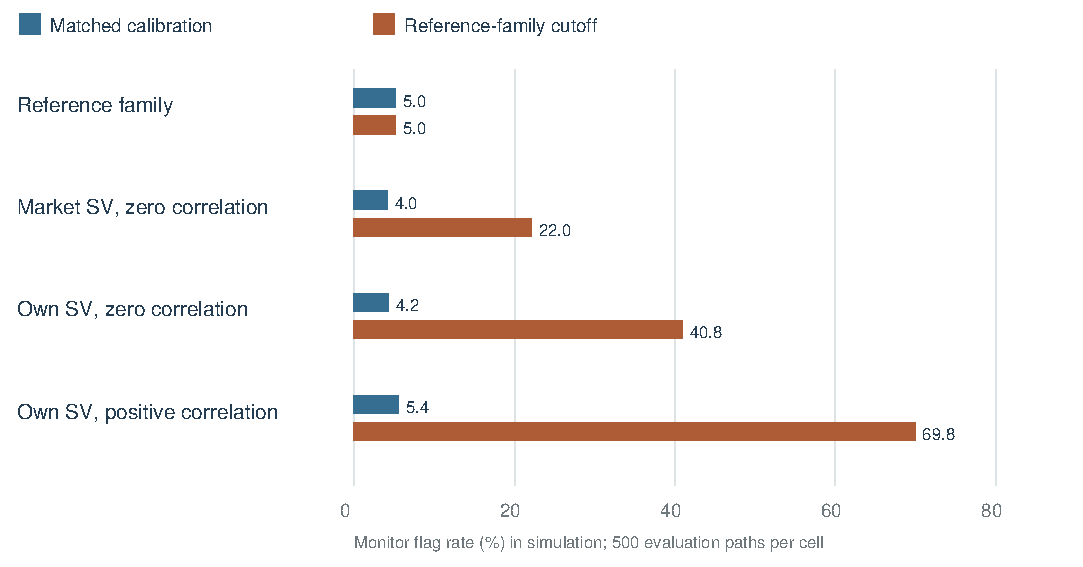
\includegraphics[width=\linewidth]{generated/calibration_transport.pdf}
\caption{The same daily monitor under matched and transported calibration.
``No level term'' is the structural simulation label; it does not claim
that all these models have the same pricing-martingale classification.
Source: experiment 055.}\label{fig:transport}
\end{figure}

This result explains why calibration is part of the method. Matched
calibration can absorb the distribution of a nuisance pattern, but the
price of doing so may be weaker separation from the alternatives. The relevant empirical question is how closely the reference library
resembles the target population in the features that drive the score.

The diffusion simulations were also compared at 10 and 50 substeps per day
using coupled increments. Fitted coefficients changed little; a later
check found four monitor alarm changes among 2,100 paired paths at fixed
coarse cutoffs, indicating relatively stable decisions at those resolutions.

\subsection{What the earlier exact-model experiments establish}
Exact constant-elasticity likelihoods offer a complementary benchmark. In a
two-exponent, four-scale catalogue, simulated null rejection was at most
0.1\% at a 5\% target. Against $p=2$, daily power rose from roughly
24--46\% over one year to 96--98\% over five years; five-minute sampling
gave nearly complete detection in the tested settings. This establishes
that level dependence can be statistically visible under strong model
restrictions.

Misspecification changes the picture. A geometric Brownian scale between
catalogue points was flagged 24\% of the time in a five-minute experiment.
Allowing a continuous Gaussian scale fixed that particular problem, but
repeated variance regimes broke the expanded procedure on daily panels.
Permitting switch dates restored validity within the switch model while
reducing power: in one five-year $p=1.5$ comparison, 44.7\% became 17.3\%
with a single admitted midpoint and 2.1\% when the middle 80\% of dates
were admitted. The experiment quantifies the sensitivity lost as that
particular comparison model becomes more flexible.

At high frequency, a declared intraday clock can preserve substantial
in-model power. Rounding and observation noise require their own
likelihood treatment. The lab's exact hidden-price filter avoids a
worst-case penalty at every rounded observation; certified calculations
were within roughly one log-likelihood unit of the ideal on simulated
\$5 geometric-Brownian null records of 30 and 125 days at cent ticks.
This is a result for that observation model, separate from the empirical
Student-$t$ replays.
\source{experiments 019, 022, 025--028; claims 033--038,
055, and 059. See the research map for the distinction between experiments
and formal results}

\section{Daily observations in the market}\label{sec:dailyresults}
The daily evidence has three roles: comparing historical episodes with calm
records; observing alarm behavior in a broader population; and checking
whether different constructions continue to differ after calibration.
Forecasting later outcomes is an additional exercise, considered after the
alarm results.

\subsection{Data and comparison design}
The early historical collection includes the dot-com period, financial and
housing-related names around 2007, and later run-ups. Separate records add
collapsed names where free data could be recovered. The broader study uses
the pinned current S\&P 500 constituents, with 416,380 overlapping windows
of 13, 24, or 72 months in the earlier analysis. It is unselected with
respect to the score, but not a historical point-in-time investment
universe.

Missing delisted names can change results in either direction. Failed firms
remove collapses; acquired firms can remove run-ups ending in takeover
premiums. The lab recovered only part of a union of public deletion lists,
with especially poor historical coverage before 2008. The direction of
survivorship bias is therefore ambiguous. Adjusted-close replays also use
a retrospective corporate-action record.

The daily market-scale replay uses monthly launches, 252 prior returns,
and a 252-session scored suffix. It starts in 1994 because SPY history and
the initial scale/training requirements constrain earlier dates. At each
launch, references are earlier completed universe records selected by a
calm-start predicate on training volatility and drawdown. Up to 499 are
taken in a fixed score-blind order, at most one per name per quarter.
The batch statistic, monitor maximum, and GSADF maximum receive separate
rank cutoffs from those same references.

\subsection{The daily market-scale signal changes the alarm pattern}
Among 150,519 universe launches with a finite calibration cutoff, the batch
statistic flags 2.91\%, the monitor 3.05\%, and GSADF 6.86\%. Including
3,197 early launches without a usable reference gives 153,716 launches and
the slightly lower rates used in Table~\ref{tab:daily}. Keeping these
denominators separate prevents the absence of a cutoff from appearing to
be successful non-rejection.

\begin{table}[htbp]\centering\small
\begin{tabularx}{\linewidth}{@{}Yrrrrr@{}}\toprule
Launch period & Launches & Batch & Monitor & GSADF & Calm batch\\
\midrule
\tablerows{generated/daily_periods.tex}
\bottomrule\end{tabularx}
\caption{Daily real-data flag rates (\%). ``Calm batch'' restricts to
calm-start records. Periods classify the launch, with the following year
scored. Early no-reference launches remain in this table. Source:
experiment 056.}\label{tab:daily}
\end{table}

\begin{figure}[htbp]\centering
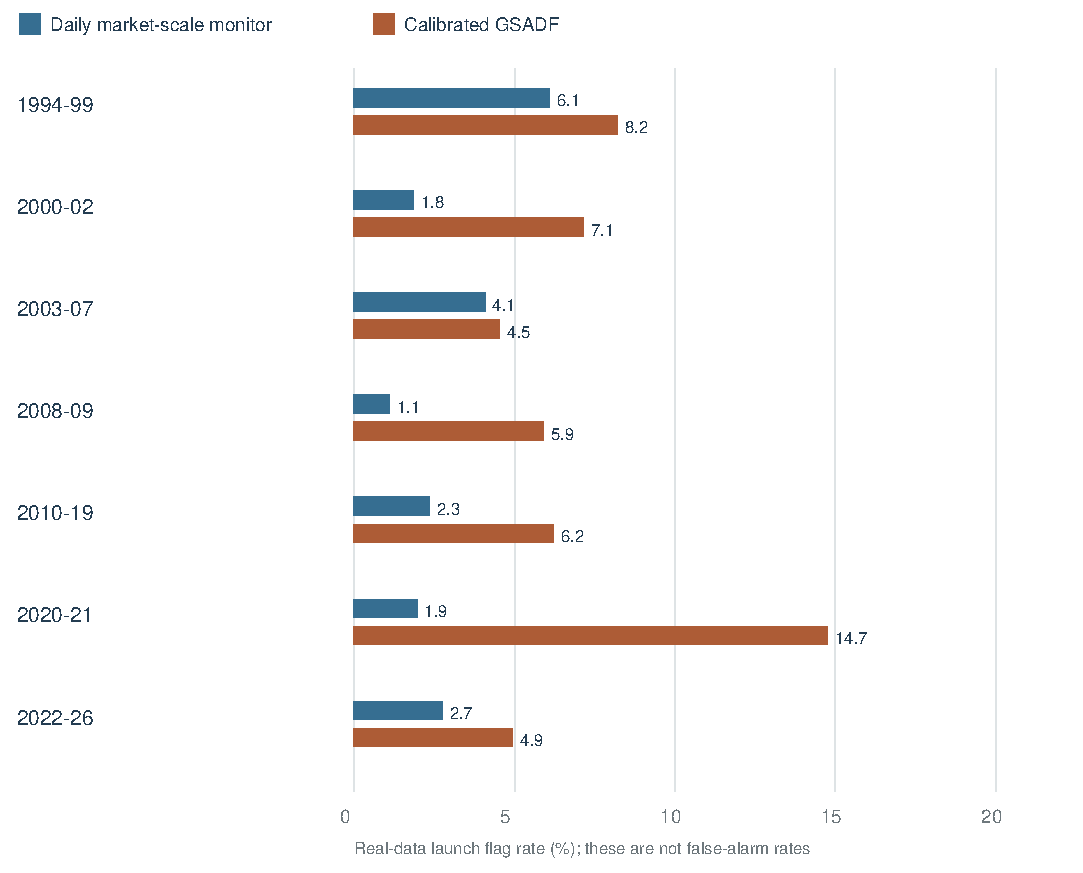
\includegraphics[width=0.95\linewidth]{generated/daily_flags.pdf}
\caption{Daily monitor and calibrated GSADF rates by launch cohort. Both
procedures use the same universe and earlier reference records. Source: experiment 056.}\label{fig:daily}
\end{figure}

The daily signal remains sparse in the three turbulent launch cohorts.
Batch rates are 1.8\% in 2000--02, 0.9\% in 2008--09, and 1.4\% in
2020--21; monitor rates are 1.8\%, 1.1\%, and 1.9\%. GSADF rates are
7.1\%, 5.9\%, and 14.7\%. The daily procedure's response therefore differs
substantially from an explosive-price screen, consistent with its design
of adjusting for common variance movements. The 1990s calm-start rate is
higher, so the contrast is specific to these cohorts.

\subsection{Homebuilders: a coherent early sector signal}\label{sec:homebuilders}
The four homebuilders provide the clearest daily case study. The monitor
flags D.R. Horton and Lennar in December 2003, then Pulte and Toll Brothers
in January 2004. Their respective price peaks occur in July 2005. All four
alarms precede the peaks by 377--411 trading sessions, a remarkably similar
lead across the sector. GSADF flags only Toll Brothers, 112 sessions before
its peak.

\begin{table}[htbp]\centering\small
\begin{tabularx}{\linewidth}{@{}Yllrr@{}}\toprule
Name & First daily alarm & Price peak & Daily lead & GSADF lead\\
\midrule
\tablerows{generated/homebuilders.tex}
\bottomrule\end{tabularx}
\caption{Homebuilder alarms in the registered 2003--08 records. Leads are
trading sessions before each record's price maximum; a dash denotes no
alarm. Source: experiment 056.}\label{tab:homebuilders}
\end{table}

This is evidence of a shared developing price--variance pattern well before
the sector's peak. For monitoring, identifying that development is a
useful distinct objective from predicting the date of reversal. The table
records first crossings; it does not measure the subsequent persistence or
intensification of the signal.

Across the wider collection, the daily monitor alarms before the peak on
15 of 30 supported consensus-positive records, against 14 for GSADF; on
the collapsed-name collection, the counts are 4 of 9 against 3. On 18 recent
narrative records, they are 7 against 10. The median pre-peak consensus lead
is 377 sessions versus 142 for GSADF. Results differ within financials:
BAC, JPM, AIG, and FNMA trigger after their peaks, while Lehman and
Countrywide trigger 107 and 833 sessions before theirs.

Two comparison conventions matter. Across consensus-negative records,
4.8\% of launches alarm and 35 of 91 records contain at least one alarm;
monthly relaunching creates more opportunities than a single launch.
GSADF also uses prior-inclusive history: 315 of its 650 alarmed episode
launches cross on the first scored day. These are comparisons of the
specified operational procedures.
\source{experiment 056, including its denominator and timing readings}

\subsection{How this differs from the repaired own-state score}
The earlier repaired daily score used a stock-specific volatility state.
On 10,000 universe windows, its empirical rate was 4.9\%, but yearly rates
ranged from about 1.4\% to 16.2\%. It flagged only 3 of the 33 requested
consensus positives, while flagging 20 of 103 calm controls; three non-US positive
records lacked complete histories on the imposed US calendar. Its consensus ranking had an AUC of 0.34,
with an interval containing 0.5. That repair had little episode discrimination under its specified design.

On common windows, the market-scale statistic has a rank correlation of
about 0.34 with that own-state score. Their distinct outputs show that changing the background-state treatment
materially changes the measurement.
\source{experiments 051 and 056}

\subsection{What the earlier alarms contain}
An audit of 185 flags from the earlier historical comparisons found that
156 survived a declared jump filter, including 137 of 153 explosive-root
flags. In daily records, rising volatility through the window was the
more distinctive feature: 69\% of flags exceeded the controls' 95th
percentile of the second-half/first-half volatility ratio. Removing jumps
increased the daily calm GSADF rate from 19.4\% to 25.2\%. This helps
explain why background variance and empirical calibration matter more than
simply deleting extreme returns in these comparisons.
\source{experiment 041; the audit concerns the earlier scores, not a new
jump-filter evaluation of the daily market-scale monitor}

\subsection{Implied volatility as a different background scale}
A separate construction used a lagged VIX or VXN value to scale a declared
Gaussian null. In simulation it had daily power against level dependence
not already reflected in that scale; dependence tracked by the supplied
scale was absorbed. In real SPX and NDX windows the registered scores were
silent, including the named historical episodes, apart from a few
crossings in a narrower sensitivity band. Some variance ratios fell outside
the declared band, and VIX before 22 September 2003 is a retrospective
backcast, making the earlier SPX windows reconstructed-scale analyses.
A separate stricter as-of design was withdrawn before scoring. The daily
market-scale method above uses a different background adjustment.
\source{claim 042; experiments 043 and 047}

\section{What five-minute data add}\label{sec:intradayresults}
The intraday evidence first examines the pattern, then evaluates the
specified monitor. These are different exercises: a coefficient estimated
on a whole retrospectively chosen episode is not an alarm available at its
beginning.

\subsection{Within-session variance behavior}
On the descriptive collection, the median within-day variance exponent is
$2.35$ for four meme-stock records and $1.48$ for 20 narrative-name
records. Four growth-name records have median $-3.59$; calm Dow members
have median $-5.94$. Most index estimates hit the lower search boundary
of $-20$, which is a numerical boundary, not an estimate beyond that
boundary. The meme records show positive fitted effects, while the growth
collection and some prominent narrative names show the usual negative
direction.

The pattern is less pronounced when one isolates hindsight-defined
run-up segments, and the estimates also respond to return--volatility
correlation in simulation. The empirical result is a difference in measured price--variance behavior
across these groups, encompassing both local-level and correlated-volatility
interpretations discussed in Section~\ref{sec:sin}.
\source{experiments 052--053; model-based curvature errors for the
within-day fits are distinct from empirical calibration}

\subsection{A retrospective replay of the monitor}
The specified monitor is calibrated on 499 calm-start references from
2017--18, all completed before targets begin in February 2019. It then
replays each 21-session launch with an assumed one-minute availability
delay. GSADF is evaluated at each daily close using the 252 prior closes
and the monitored sessions so far, with its own cutoff fitted to the
same reference IDs.

\begin{table}[htbp]\centering\small
\begin{tabularx}{\linewidth}{@{}Yrrr@{}}\toprule
Records & Launches & Intraday monitor & GSADF\\
\midrule
\tablerows{generated/intraday.tex}
\bottomrule\end{tabularx}
\caption{Launches with an alarm within the 21-session horizon (\%). The
run-up denominator retains training failures. The control rows reuse
name-launches across episode windows and are descriptive. Source:
experiment 054.}\label{tab:intraday}
\end{table}

The intraday monitor alarms on 46.2\% of meme-stock launches. Across all
run-up records the rate is 19.6\%. GSADF alarms
more often on these episodes and on none of the selected calm controls.
Of 29 run-up records, the monitor alarms strictly before the peak on 14,
GSADF on 20, with one additional GSADF alarm on the peak date. The
monitor's median pre-peak lead is 142 sessions, compared with 57.5 for
GSADF. Seven monitor alarms precede the defined run-up onset; only seven
fall between onset and peak.

There are important availability and timing differences. Of 449 run-up
launches, 109 fail before fitting because fewer than 200 prior sessions
have at least 70 bars. Seven records never obtain a successful launch.
The failures remain in the rates. GSADF uses the available daily history,
and 163 of its 182 alarmed positive launches cross on the first monitored
session. Thus the table compares procedures that can be deployed under
the declared rules, with GSADF benefiting from more daily history at launch.

The calm-control table has 1,127 weighted entries but only 610 distinct
name-launches. The monitor alarms on 30 of those distinct launches,
4.9\%; the weighting in the displayed table yields different subgroup
rates. Inference must account for repeated names and dates. In an
unselected 100-name draw, the monitor alarms on 5.0\% of 8,600 launches,
versus 5.4\% for GSADF, with its own annual rate varying from 2.3\% to
9.8\%. These frequencies describe the broad-draw population under the
fixed reference calibration.

The direct daily/intraday comparison also favors the faster observations
for early recognition. Among the 29 common run-up records, both monitors
alarm somewhere in 14, with the intraday alarm earlier in 13 of those.
Five records have only a daily alarm, six only an intraday alarm, and four
neither. Counting strictly pre-peak alarms, the totals are 13 daily and 14
intraday. These are the registered record definitions; three names have
different peak dates in the two source experiments.
\source{experiment 056, comparison with experiment 054}

\subsection{Incremental out-of-sample drawdown information}
The intraday score supplies the first positive incremental out-of-sample
drawdown result in this sequence of lab scores. Adding it to GSADF raises
predictive $R^2$ from 1.05\% to 1.39\% at 63 sessions and from 1.49\% to
1.74\% at 126 sessions. Thus the intraday statistic contains information
that the explosive-root score alone leaves out of these fitted forecasts.

Regressions use within-launch-date ranks, an intercept, and either or both
scores. Outcomes start after the completed scoring window. Coefficients
are trained on records whose outcomes end before 2023 and evaluated on
launches from 2023 onward.

\begin{table}[htbp]\centering
\begin{tabular}{@{}rrrr@{}}\toprule
Forward sessions & Intraday alone & GSADF alone & Combined\\
\midrule
\tablerows{generated/forecast.tex}
\bottomrule\end{tabular}
\caption{Out-of-sample $R^2$ (\%) for maximum drawdown, relative to the
training mean. The rows concern completed-window scores, not first
alarms. Source: experiment 054.}\label{tab:forecast}
\end{table}

The gains of 0.34 and 0.25 percentage points are point estimates; paired
uncertainty for the improvements was not computed. These score-only
regressions also leave open how much information survives controls for
realized volatility and momentum. This is the scope of the forecasting
finding, which is supplementary to the measurement and alarm results.
Neither score demonstrates return predictability in this exercise. The
daily market-scale score's drawdown $R^2$ is much smaller, approximately
0.03--0.16\%, with no demonstrated useful incremental gain over GSADF.

\section{Reading and using an alarm}\label{sec:use}
The proposed signals answer a conditional measurement question. An alarm
means that the fitted positive-level alternative accumulated unusually
large evidence relative to the declared comparison model and reference
records. It is useful to inspect the estimated level pattern, background
scale, data support, and the behavior of alternative calibrations together.
A large raw likelihood contrast with an unusual reference history is a
different finding from a stable contrast across several predeclared
reference choices.

The daily and intraday results suggest complementary descriptions. The
daily market-scale construction produces relatively sparse alarms and
has demonstrable model-based power when the market proxy tracks the
nuisance. The intraday construction detects within-session patterns in
some speculative episodes and adds out-of-sample drawdown information.
GSADF remains the stronger general episode alarm in the intraday
comparison. The new scores contribute different measurements: selective
daily patterns and an intraday component that improves the combined forecast.

For ongoing monitoring, two further results from the research matter.
First, repeatedly relaunching a monitor changes the error event. The
exact-model framework can fund declared or adaptive restarts from one
budget; it cannot discard unfavorable evidence and restart for free.
Second, dependence across names does not invalidate e-BH when genuine
e-values are supplied, but it does not make an empirical score an e-value.
Reviewer simulations of pooled forecasts found no improvement over per-name
alternatives. Experiment 029 likewise found essentially no detection gain
from selecting a cross-sectional clock within its specified model; outside
that model, selection could damage false-discovery control.

The construction of an exact filter for rounded prices is another useful
methodological result. It treats the hidden efficient price jointly across
the record instead of paying an independent worst-case penalty at each
observation. That result belongs to an exact observation model. Applying
it to recorded trade closes with different noise and rounding mechanisms
requires a new model check, not merely a finer sampling interval.


\partopening{Rebalancing and Traded Funds}{part:funds}
{How finite trading, costs, and liquidation change the expectation shortfall.}

\section{Finite rebalancing changes the classification}\label{sec:finitefunds}
The continuous-exposure result is not automatically a theorem about an
exchange-traded fund that resets its exposure once a day. Between reset
dates, the elementary contract holds fixed shares and a cash position.
This distinction changes the martingale classification even before fees,
financing, or tracking error are introduced.

Let $X$ be a continuous nonnegative $Q$-local martingale with $X_0=1$.
Over one holding interval, normalized gross wealth at exposure $\pi$ is
\begin{equation}\label{eq:oneholding}
 G_t^\pi=1-\pi+\pi X_t.
\end{equation}
Writing $\delta_T=1-\E_Q[X_T]$, linearity gives
\begin{equation}\label{eq:signedgap}
 1-\E_Q[G_T^\pi]=\pi\delta_T.
\end{equation}
For $\pi<0$ this is a negative signed gap when the underlying is strict.
It is not a negative bubble in a nonnegative asset: the affine contract
can itself become negative. Limited liability needs an additional rule.

\subsection{Finite grids with exposure between zero and one}
For a finite deterministic grid $0=t_0<\cdots<t_N=T$, define
\begin{equation}\label{eq:gridwealth}
 W_t=W_{t_i}\left(1-\pi+\pi\frac{X_t}{X_{t_i}}\right),
 \qquad t_i\leq t\leq t_{i+1},\quad X_{t_i}>0.
\end{equation}
When $X_{t_i}=0$, keep the remaining wealth in cash. For $0<\pi\leq1$,
the factors and the wealth remain nonnegative.

\begin{proposition}[Finite-grid inheritance]\label{prop:grid}
For $0<\pi\leq1$ and every finite grid, $W$ is a nonnegative continuous
local martingale and is a true martingale on $[0,T]$ exactly when $X$ is.
If $X$ is strict on that horizon, so is $W$.
\end{proposition}

The mechanism is the accumulated conditional expectation loss of each
holding. Define
$A_i=X_{t_i}-\E_Q[X_{t_{i+1}}\mid\mathcal F_{t_i}]\geq0$ and
$h_i=\pi W_{t_i}/X_{t_i}$ where the denominator is positive, zero
otherwise. Then
\begin{equation}\label{eq:lossdecomp}
 1-\E_Q[W_T]=\sum_{i=0}^{N-1}\E_Q[h_i A_i].
\end{equation}
Each summand is nonnegative. If $X$ is a martingale, every $A_i$ vanishes.
Conversely, induction gives a lower bound on the holding where $A_i$ can
be nonzero, and
$1-\E_Q[W_T]\geq\pi^N\delta_T$. This proves inheritance. The bound
can be extremely small and is generally useful for classification rather
than for monetary estimation.

The two examples in Part~\ref{part:theory} now become a comparison of
trading rules.
\begin{table}[htbp]\centering\small
\begin{tabularx}{\linewidth}{@{}YYYY@{}}\toprule
Underlying, $\pi=1/4$ & Asset & Every finite grid & Continuous wealth\\
\midrule
Absorbed Brownian, $\sigma=1$ & Martingale & Martingale & Strict\\
Reciprocal-Bessel type, $\sigma=x^2$ & Strict & Strict & Martingale\\
\bottomrule\end{tabularx}
\caption{The discrete/continuous reversal under the stated wealth and
post-default conventions. These are pricing-measure classifications.}
\label{tab:reversal}
\end{table}

At default, a finite-grid fund preserves the cash fraction left from the
last rebalance. The continuous model keeps replenishing the risky
fraction as the price approaches zero. In the absorbed Brownian example,
every finite-grid terminal mean is one while the continuous mean is
smaller, so the terminal values cannot converge in $L^1$. This does not
by itself rule out weaker modes of convergence through absorption.
\source{claims 004, 005, and 001. The stochastic inputs are finite trading,
bounded stopping, and the nonnegative-local-martingale supermartingale property}

\subsection{Refinement and the size of the discrepancy}
Away from zero, standard stability of stochastic differential equations
gives convergence of the grid recursion to the stochastic exponential as
the mesh shrinks \cite{emery1979lipschitz}. Localizing to
$X\in(1/m,m)$ gives uniform convergence in probability on a finite
horizon. If $X$ stays strictly positive throughout the horizon, the stop
can be removed. The stability theorem supplies the path-convergence step.

Path convergence does not alone ensure convergence of expectations of
unbounded payoffs. Bounded Lipschitz functionals, including puts on
nonnegative wealth, have converging expectations. Calls require additional
tail control. For $0\leq\pi\leq1$ and
$Q(X_t>0\text{ for all }t\in[0,T])=1$, a mean-one continuous limit
supplies that control automatically:
\begin{equation}\label{eq:meanone}
 \E_Q[V_T^\pi]=1\quad\Longrightarrow\quad
 \E_Q|W_T^{(n)}-V_T^\pi|\longrightarrow0.
\end{equation}
Fatou's lemma and the bound $\E_Q[W_T^{(n)}]\leq1$ force the means to
converge to one; the nonnegative shortfall then gives $L^1$ convergence.
All Lipschitz payoff expectation prices, calls included, converge.

For $\sigma=x^2$ and $\pi=1/4$, every finite-grid fund is strict yet its
defect tends to zero. Binary classification can therefore differ at every
finite frequency while the valuation discrepancy disappears. When the
continuous limit is strict, the existing result gives only a one-sided
bound on the limiting defect, not full convergence. A numerical study at
$\pi=3/4$ finds means approximately $0.786$, $0.819$, and $0.833$ for
4, 64, and 1,008 intervals, approaching the continuous value $0.8465$.
That pattern is evidence in one model; it cannot exclude probability mass
in paths too rare for the numerical calculation to resolve.
\source{claims 007 and 009; experiment 012}

\section{Leverage, inverse exposure, and liquidation}\label{sec:liquidation}
For $\pi>1$, a sufficiently large decline makes
\eqref{eq:oneholding} negative. For $\pi<0$, a sufficiently large rise does
the same. A model of a nonnegative fund must say what happens at that
point. Resetting the exposure at the next date is not enough to specify
limited liability between dates.

\subsection{Inverse funds under an explicit floor rule}
Let $W$ now be the signed finite-grid recursion at $\pi<0$. Fix
$0\leq a<1$ and liquidate into cash at the first continuous crossing
below the floor $a$, capped at $T$. By continuity, wealth at an actual
crossing is $a$. Denote stopped wealth by $H^a$. On a grid with $N$
intervals,
\begin{equation}\label{eq:inversebound}
 a\leq H_t^a\leq(1-\pi)^N.
\end{equation}
A bounded local martingale is a uniformly integrable martingale.
Thus this finite-grid, continuously liquidated inverse fund has no
defect, even when its underlying is strict.

For example, at $\pi=-1$ on one interval, liquidating when $X$ first
exceeds $3/2$ preserves wealth between $1/2$ and $2$. The underlying
$\mathrm{d}X=X^2\mathrm{d}W$ can be strict while the liquidated inverse
contract is a martingale. This is an implication of the contract rule,
not evidence that inverse exposure removes every economically relevant
risk.

\subsection{Leveraged-long funds}
For $\pi>1$, impose the same floor rule and write
$d_H=1-\E_Q[H_T^a]$. The lab establishes
\begin{equation}\label{eq:longbound}
 a\leq H_t^a\leq a+\pi^N X_t,
 \qquad 0\leq d_H\leq1-a,
 \qquad d_H\leq\pi^N\delta_T.
\end{equation}
Hence a true-martingale underlying gives a true-martingale liquidated
fund. A positive fund defect implies a positive underlying defect, but
the converse is not established. Since $\pi^N$ grows rapidly, the
quantitative lower bound $\delta_T\geq d_H/\pi^N$ is weak at daily
rebalancing frequencies.

In the registered simulations, leveraged-long funds over two strict
underlyings retain defects of roughly 0.40--0.96 at daily rebalancing
for exposures 1.5--3 with a zero floor, and 0.36--0.50 with a half-wealth
floor. Inverse funds over the strict underlyings are consistent with zero.
High-leverage geometric-Brownian controls are less stable: some inverse
cells are unresolved and the long controls at exposure three are fragile
individually. The large long-fund effects are results for these chosen
models and floor rules.
\source{claims 011 and 018; experiments 017--018}

\subsection{Costs are not a bubble}
If terminal net wealth is $Y_T=W_T-c_T+e_T$, where costs have expected
value $d_T$ under $Q$ and $\E_Q|e_T|\leq\varepsilon$, then
\begin{equation}\label{eq:cost}
 \left|(1-\E_Q[Y_T])-(1-\E_Q[W_T])-d_T\right|\leq\varepsilon.
\end{equation}
Expense, borrowing, and financing terms can be incorporated into the
one-interval return accounting, following the leveraged-fund framework
of Avellaneda and Zhang \cite{avellaneda2009path}. A deterministic fee
can lower expected net wealth without any strict-local-martingale
mechanism. An expected tracking bound under $P$ does not automatically
provide the required bound under $Q$.

The measured ETF data put a scale on these adjustments. Across eight
leveraged and inverse funds on QQQ and SPY, leveraged-long funds lose an
additional 0.6--1.7\% per year beyond the expense ratio, and inverse funds
0.1--1.1\%, measured against the total-return underlying. Reported standard
errors are 0.1--0.4 percentage points per year. Using a price index instead
would misread distributions as a cost. This is useful return accounting:
it separates ordinary financing and tracking effects from the expectation
shortfall studied in the theoretical model.
\source{claim 004; experiment 007}

\section{What discrete monitoring misses}\label{sec:monitorfloor}
Liquidation is path dependent. A simulated path can cross a boundary and
recover between observations. A program that looks only at observation
times can keep a fund alive after the continuously monitored contract
has terminated.

\begin{figure}[htbp]\centering
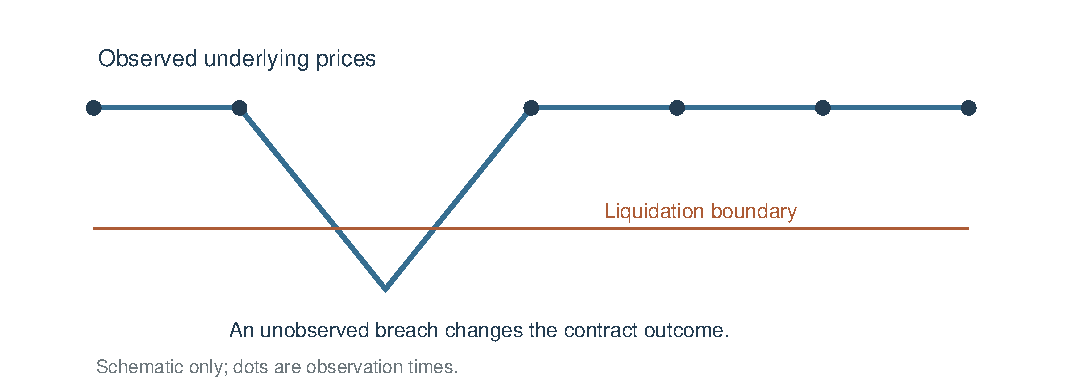
\includegraphics[width=\linewidth]{generated/missed_liquidation.pdf}
\caption{A boundary breach can be invisible at every observation time.
This is an explanatory schematic, not a simulated or historical record.}
\label{fig:floor}
\end{figure}

For monitoring times $F$ containing all rebalancing dates and $T$, define
a numerical quantity $Z_F$: if a sampled value of the signed recursion
is below $a$, replace terminal wealth by $a$; otherwise keep $W_T$.
This clipping is an artificial cash adjustment, not an executable trading
strategy. It has the useful pathwise property
\begin{equation}\label{eq:clip}
 a\leq H_T^a\leq Z_F,\qquad
 1-\E_Q[Z_F]\leq d_H.
\end{equation}
Adding monitoring times can only decrease $Z_F$. On a fixed rebalancing
grid, dense monitoring gives $L^1$ convergence to continuously
liquidated wealth under the stated models.

There is no uniform error rate based on the mesh alone over all
continuous paths. For any finite set of monitoring times, insert an
unobserved downward excursion in a gap. With one interval, $\pi=2$,
and $a=1/2$, a path observed at $X=1$ but dipping to $X=1/2$ in between
has $Z_F=1$ and liquidated terminal wealth $H_T^a=1/2$. Continuity
alone places no bound on how narrow the excursion can be.

This result gives a constructive numerical lesson. The particular clipped
quantity bounds the defect from below in expectation; freezing wealth at
the first sampled overshoot generally does not. A positive Monte Carlo
estimate still has sampling and discretization error, so it is evidence
for a positive lower bound, not a proof of its sign. The fund simulations
use this distinction to check the direction of monitoring bias.
\source{claim 020; experiment 018}

\partopening{Options and Constituent Information}{part:options}
{What additional contracts reveal, and which valuation assumptions make that possible.}

\section{Option prices do not have a unique bubble interpretation}\label{sec:optionrules}
The option results explain how additional contracts can constrain a
valuation amount. The practical difficulty appears in the observed quotes:
on the sampled end-of-day SPY chains, the largest-strike calls at one to
three months sit at the one-cent floor on most dates, at median strikes
1.07--1.41 times spot. The available far wing is therefore measured only to
the tick. Reading such quotes as a bubble bound can produce a very small
number largely determined by the pricing convention and quote resolution.
\source{experiment 014}

The central issue is whether the observed call represents an expectation
price, a parity-restoring price, or an exercise value. Assuming that a call
carries the defect and then reading a tiny quote as evidence of its absence
makes the conclusion depend on the premise being assessed. The results below
are consequently valuation identities and bounds under named conventions;
the research did not obtain a usable market bubble test from these quotes.
The algebra is nevertheless informative about which observations would
constrain a defect and which can leave it hidden.

Normalize spot to one, take zero rates and dividends, and fix a common
pricing law with $m=\E_Q[X_T]$ and $\delta=1-m$. European expectation
prices satisfy
\begin{equation}\label{eq:parityexpect}
 c(K)=\E_Q[(X_T-K)^+],\quad p(K)=\E_Q[(K-X_T)^+],
 \qquad c(K)-p(K)=m-K.
\end{equation}
Thus $1-K-c+p=\delta$. Under another declared rule, leave the put at
$p$ and set the call to $C=c+\delta$. Then $1-K-C+p=0$ even when
$\delta>0$. This second rule restores ordinary parity.

The distinction builds on the strict-local-martingale option literature.
Cox and Hobson explain how parity and exercise values depend on the
admissible trading strategies \cite{cox2005local}.
Carr, Fisher, and Ruf obtain parity restoration from their
joint-superreplication setting \cite{carr2012hedging}; it is not a
universal conclusion that market calls follow that rule. The lab uses the
two rules as explicit alternatives and works out their implications for
inference. Calling both simply ``risk-neutral option prices'' would hide
the assumption that determines the answer.

\subsection{Exercise value and the parity residual}
For the corresponding continuously exercisable American call, the lab's
localization argument gives $A_Q\geq c+\delta$. Write
$A_Q=c+\delta+u_A$, where $u_A\geq0$ denotes any excess over that lower
bound. With a European expectation put in every row:
\begin{table}[htbp]\centering\small
\begin{tabularx}{\linewidth}{@{}YllY@{}}\toprule
Call convention & Call value & $1-K-C+p$ & Reading\\
\midrule
European expectation & $c$ & $\delta$ & Residual equals the defect\\
European parity-restoring & $c+\delta$ & $0$ & A defect can be hidden by parity\\
American exercise & $c+\delta+u_A$ & $-u_A$ & Residual concerns exercise excess\\
\bottomrule\end{tabularx}
\caption{Residuals under declared valuation rules. The table is not a
classification algorithm for market quotes.}\label{tab:operators}
\end{table}

Contract metadata distinguish American from European exercise even if their
prices coincide. Prices alone need not distinguish valuation mechanisms:
on the equality face $u_A=0$, the parity-restored European value and the
American value agree. Replacing the put by an American put adds its own
exercise premium and changes the table. Neither a zero residual nor an
American premium alone identifies a defect without the rest of the model.

With simultaneous intervals for the relevant operator prices, one can
propagate errors through the residual and test the zero-residual
restriction. If the total call-plus-put error is bounded by $h$, a
positive residual exceeding $2h$ in the expectation model is sufficient
for rejection by a conservative lower-bound rule. That is a conditional
separation statement. A bid--ask spread by itself does not establish the
required coverage of a specified pricing operator.
\source{claims 014 and 017; the D31 option-observables design. This
design contains no real-data option test}

\section{Which option observations are informative?}\label{sec:optioninfo}
\subsection{The lowest strike matters}
Suppose only expectation-priced calls are observed at finitely many
strikes $K_1<\cdots<K_r$, all at or above normalized spot one. If their
prices are compatible with a nonnegative terminal law of mean at most
one, then they are also compatible with a terminal law of mean exactly
one. They cannot exclude zero defect.

The construction is simple. Starting from a compatible random variable
$X$ with mean $m<1$, compare it with $Y=\max(X,K_1)$. Every observed
call payoff is unchanged because the added mass lies below its strike.
But $\E[Y]=K_1+c(K_1)\geq1$. Mixing the two terminal laws raises the
mean to one while preserving the entire observed call panel.

This is a statement about terminal laws, not a construction of a diffusion
for every feasible law. It still makes a useful observation-design point:
adding ever-higher call strikes does not automatically identify the mean
missing below the lowest strike. An in-the-money call can exclude mean
one in this model. A matched underlying call and put identify the mean
directly through \eqref{eq:parityexpect}, conditional on expectation pricing.

The lab also constructs computable outer intervals for the defect using
call monotonicity, convex secant slopes, and quote intervals. Those
inequalities alone are not always a sharp characterization of attainable
terminal laws. Inconsistent observations must be reported as model
incompatibility, not automatically as positive bubble evidence.
\source{claim 021}

\subsection{Do options on leveraged funds add information?}
For a normalized fund, the same expectation-pricing identity yields its
defect from a call--put pair. Finite-grid inheritance then links a
positive fund defect to the underlying defect. For exposures
$0<\pi\leq1$, the quantitative link uses the factor $\pi^N$; for
liquidated long leverage it uses $\pi^N$ in the opposite inequality.
Both become weak for monetary estimation at realistic numbers of resets.

For example, $0.75^{252}$ is about $3\times10^{-32}$. An upper bound
on the fund defect divided by this factor is normally uninformative
about the underlying's defect. On the leveraged side, a positive fund
defect divided by $\pi^N$ supplies a negligible lower bound. Zero
exclusion can remain mathematically meaningful even when amount
estimation is weak, but its practical power then depends on resolving a
small residual amid costs, tracking, and quote uncertainty.

If an exact expectation-priced underlying call--put pair is already
available, it identifies the defect without fund options. Adding fund
options cannot improve on exact identification. With only underlying
out-of-the-money calls, a positive fund residual can add a restriction,
but no empirical gain specific to leverage has been demonstrated. The
inverse liquidation model in Part~\ref{part:funds} has zero fund defect
even over a strict underlying, so it cannot supply the same zero-exclusion
logic.
\source{claims 014, 018, and 021; no real-data fund-option detection
result is claimed}

\subsection{Continuous exercise creates another limiting distinction}
Let $G_t=\bar S_t+D_t$ be a finite continuous nonnegative
$Q$-local martingale, where $\bar S_t=d_tS_t\geq0$ and $d_t$ is a
positive deterministic continuous discount factor, bounded on $[0,T]$.
The cumulative discounted distributions $D$ are adapted, nonnegative,
nondecreasing and c\`adl\`ag, with $D_0=0$. A distribution jump may be
offset by a price drop while the gain process remains continuous. Write
$b_G(T)=G_0-\E_Q[G_T]$, and define
\[
 C_E(K,T)=\E_Q[(\bar S_T-d_TK)^+],\qquad
 A_Q(K,T)=\sup_{\tau\leq T}\E_Q[(\bar S_\tau-d_\tau K)^+],
\]
where the supremum includes every stopping time in $[0,T]$.
For this continuously exercisable American call,
localization at high gain levels and bounded convergence of the capped
payoff component give
\begin{equation}\label{eq:american}
 A_Q(K,T)\geq b_G(T)+C_E(K,T)\geq b_G(T).
\end{equation}
The relation between American exercise and bubbles has established
antecedents \cite{bayraktar2011strict}; it is not presented as a new
general pricing principle. The lab's treatment includes distributions
and the transfer to fixed-basket bounds.

The contrast with finite exercise is especially revealing. European
expectation calls tend to zero as $K\to\infty$. The same is true when
exercise is restricted to any fixed finite set of dates, because the
exercise payoff is bounded by a finite sum of integrable call payoffs.
Such prices therefore cannot uniformly bound a positive defect from
above as the strike increases. Continuous exercise permits stopping at
rare high levels in a way that a fixed finite exercise schedule does not.
The order of these limiting operations matters.

A tiny quoted call is consequently not an assumption-free certificate
of a tiny bubble. To use \eqref{eq:american}, the quote must provide a
justified upper bound on the specified continuous-exercise value. The
model of exercise and its relation to observed market prices are
substantive premises.

\section{From an index to its constituents}\label{sec:baskets}
For fixed positive holdings $n_i$ and a common pricing measure, let
$I_t=\sum_i n_iS_{i,t}$, $\omega_i=n_iS_{i,0}/I_0$, and
$b_i(T)=S_{i,0}-\E_Q[S_{i,T}]$. Linearity gives
\begin{equation}\label{eq:basketadd}
 b_I(T)=\sum_i n_i b_i(T),\qquad 0\leq n_i b_i(T)\leq b_I(T).
\end{equation}
This is a consequence of the definition, not a new diversification
principle. It concerns fixed holdings under one measure; a rebalanced
index needs its trading rule specified separately.

\subsection{Ordinary weights can hide all of the effect}
Suppose two names are proportional strict prices, with equal initial
weights. Their ordinary cap weights remain exactly one-half. Both can
have positive defects while neither weight declines. Thus a proposed
attribution based solely on expected losses of ordinary weights cannot
work in general.

The corrected representation uses the index share probability. Its
defining identity carries an explicit survival event up to a lifetime
$\tau^I$ \cite{kardaras2015strict}. Let
$\mu_i(t)=n_iS_{i,t}/I_t$ and
$\mu_i^\dagger(t)=\mu_i(t)\ind_{\{t<\tau^I\}}$. Then
\begin{equation}\label{eq:killed}
 \omega_i-\E_{\widetilde Q_I}[\mu_i^\dagger(T)]
       =\frac{n_i b_i(T)}{I_0},\qquad
 \sum_i\mu_i^\dagger(T)=\ind_{\{T<\tau^I\}}.
\end{equation}
These survival-adjusted, or killed, weights need not sum to one after
the lifetime. Ordinary weights do, which is why they cannot all be
supermartingales with a positive total expected loss under a single
probability. In the proportional example, all the loss is carried by
the survival factor.

The associated index hazard is also a survival-weighted mixture. If
$p_i(t)=\E_Q[S_{i,t}]/S_{i,0}$ are absolutely continuous with
$h_i=-p_i'/p_i$, then
\begin{equation}\label{eq:hazard}
 p_I=\sum_i\omega_i p_i,
 \qquad h_I=\sum_i\frac{\omega_i p_i}{p_I}h_i.
\end{equation}
The weights are not simply today's or the initial cap weights. These
are auxiliary-measure lifetimes and hazards, not directly observed
physical crash probabilities.
\source{claim 010}

\subsection{A conditional recovery formula}
Let $\nu_T$ be the pricing distribution of the terminal index. The recovery result takes this distribution as a supplied population
input. Let
$m_i(x)=\E_P[\mu_i(T)\mid I_T=x]$. If the terminal change of measure
has the form $\mathrm{d}Q/\mathrm{d}P=k_T(I_T)$, then conditioning on
the terminal index preserves the conditional mean weights. Hence
\begin{equation}\label{eq:recovery}
 \frac{n_i b_i(T)}{I_0}
   =\omega_i-\frac1{I_0}\int x m_i(x)\nu_T(\mathrm{d}x).
\end{equation}
The weaker condition that the conditional mean weights agree under
$P$ and $Q$ already suffices. The density condition is one way to imply
it, and is much stronger than loosely saying that the pricing kernel
``depends on the market.''

The formula is an identification result under that restriction, not an
estimator from one historical stock panel and today's finite option
chain. The required conditional means and pricing distribution are
population objects. The lab's estimator assumes independent physical
terminal panels and an independent supplied pricing sample; it does
not construct those inputs from overlapping historical windows.

There is a necessary compatibility check:
$0\leq\int x m_i(x)\nu_T(\mathrm{d}x)\leq n_iS_{i,0}$ for every
name. The estimated contributions summing to the index contribution
is not a check, because the identity follows automatically when the
conditional weights sum to one. This distinction is useful whenever
an attribution method appears to validate itself by matching a total.
\source{claims 016 and 044}

\subsection{What the synthetic estimation says}
The recovery estimator preserves the total on every sample and is
consistent under the stated sampling and approximation assumptions.
A histogram-based necessary-compatibility test has a conditional
finite-sample error bound with a supplied smoothness constant. In
controlled terminal-law examples, finite-sample tests detect large
violations; the fixed partitions used there do not implement an asymptotic
power construction.

In the more process-like basket example, however, the bubble contribution
is about $0.0041$ while the fixed-partition estimator bias is about
$0.0035$. Increasing the sample size does not remove fixed-range and
fixed-partition bias. No compatibility rejection was observed in the
basket cases tested. A numerical smoothness estimate gives convenient
intervals but lacks a rigorous bound; the available rigorous bound is too
large to make those intervals useful. The population identity is stronger
than this estimator's demonstrated performance.
\source{experiment 046}

\subsection{What a basket budget can and cannot identify}
Suppose an option on a tracking fund supplies a justified upper bound
$U$ on its American exercise value, and $\eta$ bounds the expected
tracking discrepancy under $Q$ relative to a frozen basket. With the
appropriate scaling $a$, the total defect is bounded by
$B_{\mathrm{cap}}=aU+\eta$. Then
\begin{equation}\label{eq:budget}
 \frac{b_i(T)}{S_{i,0}}
    \leq\frac{B_{\mathrm{cap}}}{\omega_i I_0}.
\end{equation}
The same absolute budget can give an informative relative bound for
a large constituent and a vacuous one for a tiny constituent. Tracking
under the physical measure does not supply $\eta$, and fees and basket
reconstitution can matter more than a small quoted wing call.

An upper budget alone never forces any particular name to have a
positive defect. Combined with individual intervals and a positive
lower bound on the total, the lab derives exact coordinate bounds for
the resulting box intersected by a weighted-sum constraint. That
finite-dimensional calculation is useful bookkeeping, but it cannot
create the missing monetary lower bound from a binary price-based
signal. A small positive upper bound is a tolerance certificate, not
proof of exact absence.
\source{claims 017 and 019}

\section{What the four parts establish}\label{sec:remaining}
The research gives a connected account of three practical objects: a
price--variance signal, the wealth produced by a trading rule, and an
expectation shortfall under a pricing law. The daily statistic detects
specified level alternatives substantially more often than calibrated
GSADF and identifies a coherent early pattern across the four homebuilders.
The intraday score adds drawdown information to the explosive-root
benchmark. Calibration determines the reference against which either
pattern is unusual.

The theory explains why those measurements and a valuation defect are
related but distinct. Rapidly growing local volatility and the positive
shock alignment in Sin's model provide two mechanisms. The exposure
classification shows how rebalancing can change strictness, and the
finite-grid and liquidation results explain why actual contract rules
matter. A bounded liquidated inverse fund and an unbounded leveraged-long
fund can have different expectation properties over the same underlying.

Options and constituent data then put structure on the valuation question.
A matched expectation-priced call and put determine a terminal mean;
a high-strike call panel alone can leave it unidentified. A fixed basket
adds constituent defects, while attribution needs more information than
ordinary weights. These results give the practitioner useful distinctions:
which pattern a monitor measures, which exposure a contract creates, and
which assumptions make a monetary bound informative.

\clearpage
\appendix
\section{Notation and algorithm specifications}\label{app:algorithms}
\subsection{Common notation}
\begin{longtable}{@{}L{0.20\linewidth}L{0.74\linewidth}@{}}
\toprule Symbol & Meaning\\\midrule\endhead
$P,Q$ & Physical observation law and a specified pricing measure.\\
$b_S(T)$ & Monetary defect $S_0-\E_Q[S_T]$.\\
$\delta_T$ & Defect of a price normalized to start at one.\\
$\sigma(x),p$ & Price diffusion coefficient; CEV price exponent in $\sigma(x)=\kappa x^p$.\\
$I_0,I_\infty$ & Lower and upper integrals of $x/\sigma^2(x)$.\\
$\pi$ & Portfolio exposure, not a significance level.\\
$W,V^\pi,H^a$ & Finite-grid wealth, continuous wealth, and floor-liquidated wealth.\\
$\beta$ & Full variance/price exponent; $\beta=2(p-1)$ in the CEV motivation.\\
$A_t,v_t$ & Background variance and variance including the level term.\\
$\mu,\nu$ & Return location and Student-$t$ degrees of freedom.\\
$M_t,m_t$ & Lagged market squared-return scale and its training-normalized value.\\
$h_d,c_j$ & Intraday background state for session $d$ and diurnal slot clock.\\
$\alpha$ & Per-record calibration target.\\
$n_i,\omega_i,\mu_i(t)$ & Fixed basket holdings, initial cap weights, and current cap weights.\\
$\nu_T,\eta_T$ & Index pricing distribution and its size-biased subprobability measure.\\
\bottomrule
\end{longtable}
Earlier papers and code use the letter $\beta$ for several different
objects, including the CEV price exponent, the exponent of standard
deviation, and the bubble amount. They are not identified with one another
here. Monetary defects use $b$, CEV price elasticity uses $p$, and the
statistical variance exponent uses $\beta$. The common D35 fitter used by experiments 050--051 and the D36 monitor
in experiment 054 store $\beta/2$ in the present notation. Experiments
049, 052--053, and D37 use the full variance exponent. Historical power figures quoted without an
exponent should not be used to infer a different scaling convention.

\subsection{\texorpdfstring{Student-$t$}{Student-t} density and the numerical profile}
For variance parameter $v$ and $\nu>2$, the variance-one Student-$t$
log density is
\begin{align}\label{eq:tdensity}
 \log f(r;\mu,v,\nu)
 &=\log\Gamma\!\left(\frac{\nu+1}{2}\right)
  -\log\Gamma\!\left(\frac\nu2\right)
  -\frac12\log\bigl(\pi(\nu-2)v\bigr)\notag\\
 &\quad-\frac{\nu+1}{2}
      \log\!\left(1+\frac{(r-\mu)^2}{(\nu-2)v}\right).
\end{align}
With $v_t=A_t e^{\beta x_{t-1}}$, write
$z_t=(r_t-\mu)^2/((\nu-2)A_t e^{\beta x_{t-1}})$.
The derivative of a log-density contribution is
\[
 \frac{x_{t-1}}2\left(-1+(\nu+1)\frac{z_t}{1+z_t}\right),
\]
and the second derivative is nonpositive. This concavity motivates the
half-line profile search. A boundary derivative is checked first;
otherwise the implementation doubles the search magnitude up to
$2^{30}$, then bisects a derivative bracket to width $10^{-10}$, with
at most 200 bisections and 400 objective/derivative evaluations. These
are floating-point stopping rules, not outward error enclosures.

The profile may be flat, unbounded, or unresolved. Each case has a
separate status. A failed required profile produces the failure score
$-1$, which cannot create a positive alarm; a missing required history
ends the supported prefix. An alarm already raised is not withdrawn by
a later failure. Numerical failure handling is part of the calibrated
map, not permission to remove difficult paths from the denominator.

\subsection{Daily implementation}
The daily prior fit uses $\mu\in[-0.1,0.1]$ per session,
$w\in[10^{-8},0.25]$ in daily squared-log-return units,
$g\in[0,2]$, and $\nu\in\{6,10\}$. For each $\nu$, three
deterministic starts use $g=0,1,2$. The optimizer scales $\mu,g$
linearly and $\log w$ linearly to unit intervals. It uses L-BFGS-B with
fixed tolerances, and accepts a solution only after re-evaluating a
finite objective with positive variances. Failed attempts are retained.
The selected fit is shared by every subsequent exponent.

The market proxy in \eqref{eq:marketscale} uses raw squared returns,
not centered returns, intraday integrated variance, or the target day's
SPY return. No forward filling is allowed. All 252 prior stock/scale
rows are required. The real-data reference predicate uses the last
126 training returns: stock annualized root-mean-square volatility at
most 0.30 and drawdown at most 0.15, with corresponding SPY limits
0.20 and 0.10. Reference scored suffixes must finish strictly before
the target launch. The selected reference order is a fixed hash order,
with at most one launch per symbol per quarter.

The batch score uses \eqref{eq:batch}; the monitor uses
\eqref{eq:monitor} and the same monotone bounded transformation on
positive log evidence. Each is calibrated separately from its endpoint
or its full-path maximum. With insufficient references for the rank,
the threshold is infinite. The numerical domains make the procedure
reproducible; they are not asserted to cover every true market parameter.

\subsection{Intraday implementation}
The intraday prior fit uses $\mu\in[-0.01,0.01]$ per five-minute
return, $h_{\mathrm{init}}\in[10^{-12},0.04]$, and
$\nu\in\{6,10\}$. The clock requires at least 200 prior sessions
with at least 70 finite bars and sufficient observations in each
scheduled slot; a declared whole-clock SPY fallback is used where
allowed by the protocol. A full session contributes 77 adjacent
returns from 78 bar closes. Overnight movement and the return into
the first bar are excluded.

Let $J_d$ be the supported scheduled returns of a completed session.
The common background state updates as
\[
 h_{d+1}=\lambda h_d+(1-\lambda)
       \frac1{|J_d|}\sum_{j\in J_d}\frac{(R_{d,j}-\mu)^2}{c_j},
 \qquad\lambda=2^{-1/20}.
\]
The clock and the update coefficient are frozen; the state advances
only after the session. The variance at each scored return is
\eqref{eq:intradayscale}. The mixture is accumulated over all supported
returns, even though the price anchor resets each session. Early
closes have planned-closed slots rather than fictitious zero returns.

The record is a retrospective replay of split-adjusted consolidated-tape
closes with assumed availability one minute after the bar. Bar closes
can be sub-cent even in raw data, so a cent-rounding likelihood does
not automatically describe them. The numerical method here does not
use the lab's certified rounded-price filter.

\subsection{Comparators and differences between experiments}
GSADF scans expanding and rolling subsamples for right-tailed
Dickey--Fuller evidence \cite{phillips2012multiple}. The lab reproduced
the published critical values and size tables within simulation
tolerance. The published Table 4 power comparison was not reproduced:
eight of ten cells were outside tolerance, with incompletely specified
simulation details affecting that comparison. Later monitoring comparisons evaluate running
statistics using prior-inclusive daily history. The level monitors
learn nuisance from that history but begin accumulating their scored
evidence at launch. Equal launch dates therefore do not imply equal
evidence histories.

The JKP implementation follows the volatility-tail method
\cite{jarrow2011detect}; several operational choices, including
bandwidth scaling and the decision that a fitted function is bounded,
are the lab's readings where the paper is not fully explicit. The
original licensed tick-data figures were not reproduced. Adverse
simulation and daily-data results refer to this implementation and
sampling design. They should not be described as a proof that every
tail-based method fails under its own assumptions.

The panel explosive-root method \cite{liu2022panel} and the
intraday-signal dating method \cite{obayashi2015lifetime} add further
comparisons in the research record. Their targets and data requirements
differ from the daily level statistic. We do not combine all their
rejection frequencies into a single cross-method size ranking.

\clearpage
\section{Selected derivations}\label{app:proofs}
\subsection{The endpoint calculation}
For $b_\pi(x)=\pi\sigma(x)/x$, the original diffusion has scale density
$\rho=1$ and scale $s(x)=x-c$. In the martingale criterion, infinity
is bad because $s(\infty)=\infty$. At zero, the goodness integrand is
\[
 \frac{(s(x)-s(0))b_\pi(x)^2}{\rho(x)\sigma(x)^2}
     =\frac{\pi^2}{x},
\]
which is not integrable. Both endpoints are therefore bad for positive
exposure.

The auxiliary drift is $\pi\sigma^2(x)/x$, its scale density is
$\widetilde\rho(x)=(x/c)^{-2\pi}$, and
\[
 \widetilde s(x)=
 \begin{cases}
 c^{2\pi}\dfrac{x^{1-2\pi}-c^{1-2\pi}}{1-2\pi},&\pi\ne1/2,\\[4pt]
 c\log(x/c),&\pi=1/2.
 \end{cases}
\]
For $\pi>1/2$, the scale has finite upper limit and
\[
 \frac{\widetilde s(\infty)-\widetilde s(x)}
      {\widetilde\rho(x)\sigma^2(x)}
   =\frac{x}{(2\pi-1)\sigma^2(x)}.
\]
For $0<\pi<1/2$, it has finite lower limit and the corresponding
lower integrand is $x/((1-2\pi)\sigma^2(x))$. At one-half both
scale endpoints are infinite in their respective directions. Applying
the cited endpoint criterion yields Theorem~\ref{thm:exposure}.
The integrability requirement on $b_\pi^2/\sigma^2=\pi^2/x^2$
holds on every compact subinterval of $(0,\infty)$.

\subsection{From tail completion to testing}
Let $S$ be a strict alternative under $P=Q$ and choose $n>s_0$.
Keep its coefficient below $n$ and complete it linearly above $n$.
The completed upper integral is infinite, giving a martingale null.
The original and completed laws agree until first hitting $n$ by
stopped uniqueness in law. A coupling of the stopped observations and
their continuations therefore bounds, for a test $0\leq\varphi\leq1$,
\[
 |\E_{P_n}\varphi-\E_P\varphi|
 \leq P\!\left(\sup_{t\leq T}S_t\geq n\right)
 \longrightarrow0.
\]
For finitely many paths, use the probability that any path reaches
$n$. The finite-horizon maximum is finite almost surely, so the bound
vanishes. Taking the supremum over null rejection probabilities gives
the theorem. Allowing equivalent physical measures requires the
additional change-of-measure construction in claim 006; the
$P=Q$ subfamily already proves the central obstruction.

\subsection{An honest likelihood-ratio guarantee}
Condition on a training record. Suppose $q$ is a normalized forecast
density for evaluation observations and the true conditional density
is $p_{\theta_0}$ in the admitted null family. Then
\[
 E=\frac{q(Y)}{\sup_{\theta\in\Theta_0}p_\theta(Y)}
       \leq\frac{q(Y)}{p_{\theta_0}(Y)},\qquad
 \E_{\theta_0}[E\mid\text{training}]\leq1.
\]
Markov's inequality gives a fixed-record rejection bound at
$E\geq1/\alpha$. The reasoning needs a density on the actual
observation space. For rounded records this means cell probabilities
or a filtered cell likelihood, not evaluating a continuous density
at the reported tick. Observation noise requires its conditional law
or an honest envelope as well.

For a sequential coherent model, predictable normalized forecasts
produce a likelihood-ratio martingale relative to each true null
law. A score dominated at every time by that martingale inherits its
crossing bound. The supremum in the denominator must cover the true
whole-record law, including the conditioning convention. A nuisance
estimate frozen from training does not generally equal the true
nuisance, so the real-data monitors need their empirical calibration
instead of an automatic appeal to this argument.

If $E_1,\ldots,E_m$ are genuine e-values, e-BH uses the largest
$k$ for which the $k$th largest value is at least $m/(qk)$ and
rejects the top $k$. Its expected false-discovery proportion is at
most $q$ under arbitrary dependence \cite{wang2020false}. This
does not guarantee that a realized list has false-discovery
proportion below $q$, nor justify applying the same threshold to
scores whose null expectations are unknown.

\subsection{The rank calibration bound}
Under exchangeability, the target's rank among $m+1$ records is
uniform when ties are randomized; strict exceedance of the reference
order statistic can only reduce rejection when ties are retained.
Thus the probability of exceeding the $k$th ordered reference is
at most $(m+1-k)/(m+1)\leq\alpha$. Apply the argument to a whole
path's maximum to bound a crossing within its declared horizon.
The proof does not establish exchangeability after selecting calm
reference records. That is an external property of the application.

\clearpage
\section{Research provenance and verification scope}\label{app:record}
This manuscript is an editorial synthesis of the repository's existing
claims and experiments. It neither runs new experiments nor promotes a
numerical finding to a theorem. The original research record remains
in \path{paper/PAPER.md}, the claim files, the experiment registrations,
and their code and summaries. The source version used for generated
tables and figures is recorded in
\path{manuscript/generated/provenance.json}, together with SHA-256
hashes of the input result files and bibliography registry.

\subsection{Principal mathematical sources within the project}
The following map uses stable claim IDs; theorem numbers in this
manuscript are new and do not follow the original paper's numbering.
Each claim file states its cited inputs, proof, review, and formal
counterpart.

\begin{longtable}{@{}L{0.18\linewidth}L{0.75\linewidth}@{}}
\toprule Claims & Material used here\\\midrule\endhead
001 & Two-endpoint exposure classification and absorbed-Brownian counterexample.\\
002, 003, 006 & Compatible tails, broad testing obstruction, pricing-measure
ambiguity, and the local-volatility specialization.\\
008, 012, 013, 015 & Visited-range identity, compact estimation, declared power
tails, and shared-tail occupation.\\
004, 005, 007, 009 & Holding-period accounting, finite-grid inheritance,
refinement, and convergence when the limit retains its mean.\\
011, 018, 020 & Inverse and leveraged-long liquidation, sampled monitoring bounds.\\
014, 021 & Option residual intervals and incomplete-call information.\\
010, 016, 019, 044 & Basket additivity, killed weights, conditional recovery,
dispersion sets, and synthetic estimation.\\
017 & American-call inequality, distributions, and conditional basket tolerance bounds.\\
051--058 & Exact-catalogue inference, price-law instances, e-BH, continuous
Gaussian nuisance, and earlier-window parameter declarations.\\
023--032, 059--061 & Misspecification, rounding, and jump/switch extensions.\\
033--038, 064--067 & Clocks, observation noise, exact filtering, quadrature,
and cross-sectional clock uncertainty.\\
062--063 & Pooled likelihood constructions; comparisons are reviewer
simulations in the claim files.\\
039--042, 068--070 & Sequential scores, funded restarts, predictable implied
volatility, and variance-switch profiles.\\
045 & Empirical rank calibration and its post-selection premises.\\
071--076 & Continuous-record elasticity, variation profiles, small-scale
obstruction, infinite horizons, and independent assets.\\
\bottomrule
\end{longtable}

The numerical statement about exact rounded filtering is supported by the
claim-036--038 evaluators and checks, not by the Student-$t$ monitor.
The exposure extensions use claims 074--076 and their separate checks.
They should not be confused with later experiment numbers that happen to
use similar direction labels.

\subsection{Empirical source map}
Every numbered experiment has a registration file directly in
\path{experiments/} and, when run, code and outputs in the corresponding
numbered subdirectory. A ``reproduced'' label below refers to the lab's
recorded review, not a fresh full replication performed for this manuscript.

\begin{longtable}{@{}L{0.16\linewidth}L{0.77\linewidth}@{}}
\toprule Experiments & Use in this manuscript and principal limitation\\\midrule\endhead
001, 006 & Exposure examples; numerical evidence about selected models.\\
007--009, 012 & Measured ETF costs, finite rebalancing, and convergence; expectation
convergence is not inferred from a path plot alone.\\
013 & Sampled visited-integral estimator; not the same object as the exact
continuous-path identity.\\
017--018 & Liquidated funds and clipped monitoring; numerical defect
estimates have sampling and monitoring error.\\
002--005, 015 & Comparator implementations and simulation responses; different
null targets, and original licensed data unavailable for some methods.\\
019, 022--028 & Exact catalogues, nuisance flexibility, regimes, clocks, and
rounding; guarantees stay within the stated observation laws.\\
021, 030--033 & Historical daily, collapsed-name, and hourly comparisons;
retrospective labels and incomplete free-data coverage.\\
029, 034--038 & Common clocks, nuisance resets, wider forecasts, and
restarts; no general power guarantee follows.\\
010 & Free-data survivorship: no daily series for 57 of 506 January 2020
members, 40 of 505 December 2021 members, and 27 of 503 January 2023 members.\\
032--033, 035 & Earlier hourly likelihood scores: 0 of 21 press-labelled
records versus GSADF's 18 of 21; the widened-scale GameStop flag was
jump-sensitive.\\
041 & Jump audit: 156 of 185 earlier flags survive filtering; rising
within-window volatility is the stronger daily distinction.\\
039--040, 045 & Broad universe and GSADF calibration; current constituents,
overlapping windows, selected reference records.\\
043, 047 & Implied-volatility scale; real-data silence does not verify
the scale band or identify absence of a bubble.\\
046 & Conditional basket recovery in synthetic terminal samples; fixed-bin
bias and supplied smoothness restrict the practical result.\\
049--051 & Diagnosis, repaired-score simulation, and daily replay; research
redesign and calibration transport remain relevant.\\
052--053 & Intraday description and estimator validation; coefficient
sign is not specific to a local-volatility mechanism.\\
054 & Intraday monitor replay; 499 references, 449 run-up launches,
8,600 broad-draw launches; prior-inclusive GSADF and no untouched holdout.\\
055 & Daily validation; 499 reference and 500 evaluation paths per main
null cell; partial validation and large calibration-transport effects.\\
056 & Daily replay; 153,716 reported universe launches, including 3,197
without finite calibration; one market proxy and current constituents.\\
\bottomrule
\end{longtable}

Selected numerical tables are generated directly from the result files
for experiments 040, 054, 055, and 056. The calibration-transport and
daily-cohort figures are vector plots of those same outputs. The
liquidation figure is a schematic. Other numerical summaries in prose
are transcribed from the registered reports and the original paper;
their cited experiment identifies the relevant design and scope.
The build records input hashes and checks the typeset document, but
does not refit models, regenerate market data, or rerun the simulations.

\subsection{What Lean verifies}
The project uses Lean 4 with a pinned Mathlib. Its stochastic inputs,
including diffusion existence, martingale criteria, bounded stopping,
and occupation identities, enter as explicit hypotheses where the
library does not supply the relevant theory. Selected deterministic
analysis and conditional implications are proved from those inputs.

For the exposure classification, the endpoint analysis is formalized
without stochastic assumptions beyond its explicit deterministic
setting. The wealth classification is a conditional theorem from
the stated martingale criterion and representation. Some upstream
structures have only vacuous instances because the pinned library
does not construct the needed Brownian model; others have genuine
but degenerate instances. They do not establish a nontrivial diffusion
instance or add evidence that the supplied stochastic premises hold.

The unconditional tail-completion algebra, several finite-dimensional
interval calculations, and portions of the estimator mathematics
have stronger formal coverage than the stochastic interpretations.
Conversely, some prose corollaries---such as replacing a finite
lower-endpoint integral by the event of reaching zero---use cited
stochastic results beyond their formal counterparts. The exact scope
is documented in \path{paper/PROOFMAP.md}, the original paper's
Appendix A, and \path{board/FIDELITY.md}.

Formal verification increases confidence in the statements actually
encoded. It does not establish their novelty, the fidelity of every
translation from a source, a model of actual traded contracts, or the
validity of market-data assumptions. No new Lean theorem is claimed
for this manuscript's empirical constructions.

\subsection{Literature positioning}
The mathematical results apply established martingale criteria, diffusion
analysis, share-measure constructions, and stochastic-integral facts
\cite{mijatovic2010martingale,ruf2015martingale,karatzas2015distribution,
kardaras2015strict,etheridge2018continuous}. Likelihood envelopes, e-BH,
rank calibration, and the option valuation conventions likewise have
established antecedents. The contribution lies in the exposure
classification, the precise identification results, the signal designs,
and their measured behavior. No separate novelty claim is made for the
finite-trading results.

Section~\ref{sec:literature} supplies the substantive prior-art comparison.
For this manuscript, the author versions of Cox--Hobson, Herdegen--Herrmann,
and Herdegen--Schweizer and the Federal Reserve working paper by
G\"urkaynak were retrieved and checked for the background statements cited
there. Copies and edition metadata are retained in
\path{manuscript/sources/}. In particular, the Herdegen--Herrmann citation
uses the 2017 arXiv version read here, rather than the earlier working-paper
year in the research registry. This comparison establishes the context of
the contributions; it is not an exhaustive theorem-by-theorem novelty audit.
Other references retain the repository's version years where a working
paper was used.

\clearpage
\phantomsection
\addcontentsline{toc}{section}{References}
\bibliographystyle{plainnat}
\bibliography{generated/references}
\end{document}
